%----------------------------------------------------------------------------------
\chapter{Desenvolvimento}
%----------------------------------------------------------------------------------
Baseando-se na conceituação de engenharia de \textsl{software} dada por \citeonline{SOMMERVILLE:2019}, neste capítulo é descrito o desenvolvimento do sistema, cujas etapas estão apoiadas em técnicas que vão desde sua especificação até sua evolução.

Além do presente documento, o desenvolvimento do projeto ainda pode ser acompanhado através dos outros canais de registro que fazem parte dos requisitos da disciplina, sendo eles:

\begin{itemize}
%---
    \item \textbf{Aplicação:} A aplicação do projeto já hospedada na plataforma \gls{heroku}.
    \begin{figure}[htb]
    \centering
    \caption{\href{https://app-ifriends.herokuapp.com}{Link da aplicação}}
    \qrcode{https://app-ifriends.herokuapp.com}
    \fonte{Os autores}
    \end{figure}
    \FloatBarrier
%---
    \item \textbf{Blog do projeto:} Pelo menos uma vez por semana, o blog do projeto recebe uma postagem a respeito do que foi desenvolvido naquele período. 
    
    \begin{figure}[htb]
    \centering
    \caption{\href{https://bunkabytes.blogspot.com}{Link do \textit{blog} do projeto}}
    \qrcode{https://bunkabytes.blogspot.com}
    \fonte{Os autores}
    \end{figure}
    \FloatBarrier
%---
    \item \textbf{Canal no YouTube:} Através do canal no \gls{youtube} é possível conferir as apresentações realizadas pela equipe.
    
    \begin{figure}[htb]
    \centering
    \caption{\href{https://www.youtube.com/channel/UCOJVZlclPTqngZQwPS9Fvpg}{Link do canal no \textit{Youtube}}}
    \qrcode{https://www.youtube.com/channel/UCOJVZlclPTqngZQwPS9Fvpg}
    \fonte{Os autores}
    \end{figure}
    \FloatBarrier
%---
    \item \textbf{Repositório no \textit{SVN}:} É o repositório principal do projeto, nele se encontram todos os arquivos do projeto, desde a documentação até os arquivos de desenvolvimento. 
    
    \begin{figure}[htb]
    \centering
    \caption{\href{https://svn.spo.ifsp.edu.br/svn/a6pgp/A2022-PDS-SEG/Bunka_Bytes/}{Link do repositório}}
    \qrcode{https://svn.spo.ifsp.edu.br/svn/a6pgp/A2022-PDS-SEG/Bunka_Bytes/}
    \fonte{Os autores}
    \end{figure}
    \FloatBarrier
%---
\end{itemize}

%------------------------------------------------------------
% ------------------------------------------------------------
\chapter{Materiais e Métodos}
% ------------------------------------------------------------
Segundo \citeonline{Junior:2010}, engenharia de \textsl{software} é ``um conjunto integrado de métodos e ferramentas utilizadas para especificar, projetar, implementar e manter um sistema'', e que, para tanto, reúne em si metodologias, métodos e ferramentas para que o projeto seja bem definido em todas as suas etapas, variando desde sua problemática inicial e indo até sua entrega enquanto um produto de \textsl{software}. É a partir disto, que \citeonline{Junior:2010} distingue um método de uma ferramenta:

\begin{citacao}
Um método é uma prescrição explícita de como chegar a uma atividade requerida por um modelo de ciclo de vida, visando otimizar a execução das atividades que foram especificadas. Já as ferramentas proporcionam apoio automatizado ou semi-automatizado aos métodos \cite{Junior:2010}.
\end{citacao}

Ademais, \citeonline{Junior:2010} ainda separa os métodos de desenvolvimento de sistema em três categoriais que permitem visualizar e solucionar o problema de diferentes maneiras para sua modelagem. Para a composição do presente projeto, no entanto, será utilizado como método principal a metodologia escolhida para a gestão do projeto e as ferramentas poderão ou não ser relacionadas a ela, como há de ser especificado nas próximas seções.

%-------------------------------------------------------------
\section{Ferramentas de desenvolvimento}
%-------------------------------------------------------------
Pensando no objetivo e alcance do projeto, optou-se pela criação de uma aplicação Web, que possa ser acessada de diferentes dispositivos de forma fácil, apenas tendo como requisito básico o acesso à Internet. Outros fatores considerados foram: a experiência da equipe com o formato, os recursos computacionais exigidos para tal desenvolvimento (sendo menores que para desenvolvimento de aplicações móveis) e a maior disponibilidade de conteúdos gratuitos e de fácil acesso sobre desenvolvimento Web.

De modo a desenvolver essa aplicação, considerou-se o uso da biblioteca/ecossistema JavaScript, o ReactJS com a pré-configuração do \gls{cra} para \gls{single-page}, como base para o \textsl{\gls{front-end}}, já as bibliotecas estilísticas que servem de auxílio são o \gls{react-bootstrap} e o \gls{ant}.

Além disso, para a internacionalização, faz-se uso da biblioteca de uso livre, a  \href{https://www.i18next.com}{i18n}, escrita em JavaScript e disponível como uma dependência no ReactJs. Essa biblioteca possui muitas funcionalidades e possibilidades de uso, porém a utilizamos para internacionalizar o site, com ela é possível traduzir texto para idiomas diversos, escolher a linguagem padrão do navegador do usuário e várias outras possibilidades.

Quanto ao banco de imagens da aplicação, utiliza-se o \href{https://pt-br.imgbb.com}{imgBB}, o qual é uma plataforma de hospedagem de imagens grátis, com ela é possível enviar uma requisição a \acs{api} do \href{https://pt-br.imgbb.com}{imgBB}, que junto de uma chave própria do usuário é possível fazer a inserção, edição, visualização e exclusão das fotos. Ele também fornece os \textsl{links} das imagens, possibilitando o armazenamento no banco de dados apenas dos \textsl{links} das fotos enviadas pelo usuário.

Para o \textsl{\gls{back-end}} foi considerada a linguagem Java, orientada a objetos; sua escolha foi feita pelo fato de a equipe já possuir experiência com a linguagem, além de alguns já trabalharem com ela e de também possuir uma grande comunidade ativa que disponibiliza conteúdos gratuitos que podem ajudar no desenvolvimento. Em conjunto, está em uso o \textit{Spring Boot}: \gls{framework2} Java de código aberto, aliado ao \gls{Maven} - para a automação e gerenciamento de dependências no projeto.  Já como padrão de desenvolvimento utilizado no  \textsl{\gls{back-end}}, foi aplicado o padrão \acs{mvc}, que separa o projeto em três principais camadas: \textit{model}, \textit{view} e \textit{controller}.

No entanto, como arquitetura de sistema (\autoref{Arquitetura_Rest_API}), foi escolhido utilizar a arquitetura \gls{REST API} na qual é possível separar o código \textsl{\gls{back-end}} do \textsl{\gls{front-end}} de maneira que as duas aplicações possam determinar a troca informações entre elas com requisições via protocolo \acs{http}. Esta solução também pode ser útil para escalonar a plataforma, já que a utilização de uma \acs{api} pode ser feita tanto por aplicações móveis, como para a Web.

\begin{figure}[htb]
\centering
\caption{Arquitetura REST API}
\label{Arquitetura_Rest_API}
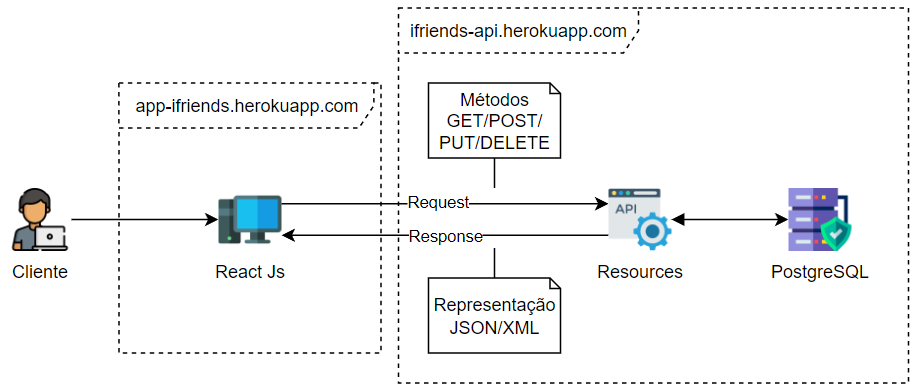
\includegraphics[width=1.0\textwidth]{anexos/Imagens_Diagramas/Arquitetura-Rest-API.png}
\fonte{Os autores.}
\end{figure}
\FloatBarrier

Quanto ao banco de dados, foi utilizado o \gls{postegreSQL}: um \acs{sgbd} popular de \acs{sql}, que serve para executar comandos no banco, como consultas, e alterações nos dados ou na estrutura.

Para hospedar a aplicação, a equipe utiliza o \gls{heroku} para hospedagem da \acs{api} e o \gls{vercel} para a interface de usuário, sendo ambas plataformas em nuvem que suportam diversas linguagens de programação e permitem a implantação, escalonamento e gerenciamento do sistema.

%-------------------------------------------------------------
\section{Ferramentas de apoio}
%-------------------------------------------------------------
Nesta seção serão especificadas as ferramentas a serem utilizadas para a estruturação e organização do sistema Web.

\begin{itemize}
\item \textbf{Notion}: Foi escolhido como plataforma de organização de projetos, pois este possui métodos de gerenciamento de equipe, fornecendo uma interface para vários desenvolvedores trabalharem utilizando o quadro de kanban, assim como o compartilhamento de arquivos, vídeos e artigos; permitindo também notificações via e-mail sobre atualizações do projeto e de reuniões marcadas, por exemplo. O quadro com todo planejamento utilizado pela equipe pode ser visto em \href{encurtador.com.br/cjvT4}{encurtador.com.br/cjvT4}.
    
\item \textbf{Discord}: Plataforma de comunicação online escolhida, por ser a mais utilizada e conhecida pelos membros da equipe. Nela é possível criar servidores privados para compartilhar informações e realizar reuniões sobre o projeto.
    
\item \textbf{Overleaf}: Para a preparação do documento de visão, será usado o \LaTeX, visto que este possui comando de padronização para documentos acadêmicos, facilitando a sua construção, juntamente, com editor Overleaf que oferece um ambiente compartilhado entre os membros da equipe. 
    
\item \textbf{Figma}: Na parte de modelagem do sistema e elaboração ideias de soluções de problemas, escolheu-se o Figma, visto que é uma ferramenta gratuita que possui diversas opções de edição.
    
\item \textbf{Visual Studio Code}: A \acs{ide} escolhida para realizar a edição de código-fonte na parte \textsl{\gls{front-end}} do sistema, por razões de ser um recurso da atualidade com possibilidades de várias adaptações de ambiente, principalmente as nossas tecnologias escolhidas.

\item \textbf{Eclipse}: A \acs{ide} escolhida para realizar a edição de código-fonte na parte \textsl{\gls{back-end}}, por motivo de facilidade que o ambiente de desenvolvimento proporciona para rodar aplicações com Java e, também, seus recursos que fazem a integração com o banco de dados.
\end{itemize}

%-------------------------------------------------------------
% -----------------------------------------------------------
\section{Métodos de gestão e desenvolvimento}
\label{metodologia agil}
% -----------------------------------------------------------
Tendo em vista a organização do projeto \gls{ifriends}, a equipe escolheu utilizar os princípios e valores do Manifesto Ágil como norteadores nos seus processos de planejamento, modelagem e desenvolvimento do projeto. Deste modo, elencou-se  o \gls{framework} Scrum como metodologia ágil como referência para o trabalho da Bunka Bytes.

%------------------------------------------------------------
\subsection{Metodologia ágil}
%------------------------------------------------------------
Segundo \citeonline{ambler2004modelagem}, o termo “metodologias ágeis” surgiu em fevereiro de 2001, quando  especialistas em processos de engenharia de \textsl{software} se reuniram e estabeleceram princípios comuns entre todas as metodologias, criando a Aliança Ágil e o estabelecimento do ``Manifesto Ágil'' \textsl{(Agile Manifesto)}.

O termo metodologia ágil consiste na otimização do tempo para a realização de determinado projeto, visando a rapidez na entrega e na qualidade, surgindo assim, como uma resposta mais leve, mais assertiva e menos custosa em relação aos métodos pesados que eram utilizados para a construção de sistemas. Nas metodologias ágeis, os processos, as ferramentas, as documentações, as negociações e os planejamentos, possuem prioridade secundária, pois os indivíduos e suas interações são considerados essências e indispensáveis \cite{sganderla2016aprimorando}.

Para isso, o manifesto determina quatro valores principais, sendo eles: o enfoque nos indivíduos e nas interações, e não nos processos ou algoritmos; a adaptação e maior flexibilidade a novos fatores decorrentes do desenvolvimento do projeto; o foco na funcionalidade do sistema e na documentação mais simples e objetiva, e por último, a preferência por um ambiente de trabalho mais colaborativo e menos burocrático  \cite{sganderla2016aprimorando}. 

Segundo \citeonline{cruz:2018}, o Scrum pode ser definido como ``um \textsl{\gls{framework}} para desenvolver e manter produtos complexos que também pode ser utilizado no gerenciamento ágil de projetos que se destinam também à criação de produtos''. Neste caso, sabida a escolha da utilização de uma metodologia ágil para o gerenciamento do presente projeto, foi decidido aplicá-la com base no Scrum e suas especificações, porém, como a finalidade do trabalho é acadêmica, resolveu-se adaptar algumas de suas características para que a metodologia pudesse ser implementada como uma referência na organização e gestão do projeto. Estas serão explicitadas mais a frente, conforme apresentadas as particularidades do \textsl{\gls{framework}}.

% Dentre as principais características do Scrum, está a divisão do desenvolvimento em ciclos repetitivos e curtos, permitindo modificações, adaptações e correções no produto de forma iterativa e incremental, o que, segundo \citeonline{cruz:2018} permite encontrar desvios mais rápido e com menos impacto. \citeonline{cruz:2018} explica que para que os processos sejam otimizados de tal forma, o Scrum possui ainda três pilares de sustentação: transparência, a inspeção e a adaptação.

Além dos pilares da metodologia, há cinco valores importantes para sua construção e prática durante um projeto: coragem, foco, comprometimento, respeito e abertura.  De acordo com \citeonline{cruz:2018} os valores do Scrum são responsáveis por reforçar os princípios do manifesto ágil, principalmente considerando o comportamento e as pessoas maiores do que os processos e ferramentas. 

%------------------------------------------------------------
\subsubsection{O quadro de kanban}
% -----------------------------------------------------------
% Segundo \citeonline{peinado2007compreendendo}, o nome kanban vem do japonês ``cartão'' e a sua origem deu-se pela seguinte razão:

% \begin{citacao}
% Este nome surgiu em razão do sistema de controle visual dos estoques de materiais, pois são frequentemente utilizados cartões para representar os contentores cheios ou vazios, estes cartões são retirados ou colocados em um quadro à medida que o material é utilizado, ou reposto
% \cite{peinado2007compreendendo}.
% \end{citacao}

% E através da implantação realizada por \citeonline{silva2012beneficios}, devido aos problemas e necessidades encontrados ao longo dos \textsl{Sprints}, houve a criação de um processo ágil, baseado nas práticas do Scrum com características do kanban:

% \begin{citacao}
% As tarefas ou itens de trabalho foram representadas através de cartões (do inglês \textsl{post-its}) fixados em um quadro (do inglês \textsl{cardwall}). 
% Esse quadro, por sua vez, era dividido em colunas que representavam as fases do fluxo de trabalho (do inglês \textsl{workflow}) da equipe. 
% As tarefas eram distribuídas sequencialmente nas colunas à medida que avançavam no fluxo de trabalho \cite{silva2012beneficios}.
% \end{citacao}

No projeto a implementação do kanban foi similar, porém todo o esquema presencial foi adaptado ao quadro remoto. Para conciliar a participação contínua da equipe, a ferramenta \textsl{Notion} é utilizada como auxiliar aos processos de organização, onde também foi possível criar os quadros de kanban do projeto. 

O quadro de kanban usado pela equipe Bunka Bytes foi dividido em dois: no primeiro, encontram-se tarefas (``cartões virtuais'') relacionadas a pendências administrativas e de documentações/mídias, apresentando 5 colunas, nas quais são representadas visualmente em qual estágio a tarefa se encontra, as colunas se classificam como ``para fazer'', ``planejamento'', ``em andamento'', ``para revisar'' e ``feito''.

Já o segundo, possui uma visão global de todas as histórias de usuário que estão sendo trabalhadas na \textsl{Sprint} atual, conforme explicado na \autoref{artefatos}, portando possui raias que variam de acordo com os estados de cada história, sendo eles divididos em: ``para fazer'', ``em andamento'', ``em revisão'', ``pronta'' e ``entregue''. Tal distinção precisou ser feita devido a uma avaliação da equipe sobre demonstrar com maior clareza os itens de \textsl{Backlog} no quadro com os atributos necessários para uma história de usuário enquanto funcionalidades do sistema (como sua pontuação, tamanho, prioridade, critérios de aceitação, descrição e aquém está atribuída), tendo em vista que estes podem ser diferentes daqueles utilizados em tarefas mais administrativas.

Desse modo, para ambos a priorização é um item em comum e deve seguir um padrão, por isso foi decidido utilizar uma classificação em ordem de prioridade para cada tarefa/história, podendo ser ``alta'', representada pela cor vermelha, ``média'', representada pela cor laranja, e ``baixa'' representada pela cor verde, tais prioridades são atribuídas às tarefas/histórias assim que a entrega é planejada.

De maneira geral, o uso do quadro de kanban é beneficial ao projeto, já que através de sua aplicação a equipe consegue conciliar de maneira clara e precisa as tarefas/histórias compartilhadas. A utilização do quadro remotamente e através do Notion, faz com que a equipe possa ainda acessá-lo de qualquer lugar, facilitando o processo de transparência dos itens e faz com que todos tenham em usas mão as atividades a serem feitas, podendo ajustá-las quando preferirem. 

%------------------------------------------------------------
\section{Gestão da equipe}
% -----------------------------------------------------------
A equipe Scrum é composta por três papéis: o \textsl{Scrum Master}, o \textsl{Product Owner} e o Time de Desenvolvimento:

\begin{citacao}
O primeiro, chamado \textsl{Scrum Master}, é considerado o responsável por garantir que o Scrum seja entendido e aplicado, para que o Time Scrum esteja aderindo os valores, as práticas e as regras do Scrum, e, portanto, trabalha como um líder ou técnico da equipe. Já o \textsl{Product Owner}, é o principal responsável pelo gerenciamento do \textsl{backlog} do produto, por garantir o valor do trabalho realizado pelo Time, e pela satisfação e atendimento das necessidades do cliente. O Time de Desenvolvimento, por outro lado, é responsável por executar o desenvolvimento e transformar o \textsl{backlog} do produto em incrementos de funcionalidades, criando um sistema pronto que possa ser entregue ao cliente \cite{cruz:2018}.
\end{citacao}

Portanto, para fins de organização, o Time de Desenvolvimento deve ser dividido em subequipes, sendo elas: desenvolvimento, design e documentação, e mídias. Nelas, estão inclusas as funções de desenvolvedores \gls{front-end} e \gls{back-end}, divididas entre os integrantes Jamilli Vitória Gioielli, José Roberto Claudinho Ferreira e Kaiky Matsumoto Silva; sendo a Jamilli e o José responsáveis por supervisionar o \gls{front-end} da aplicação, e o Kaiky pela supervisão do \gls{back-end} - que também inclui a administração do banco de dados. Porém, os três atuam de formas diretas ou indiretas em ambas as partes do desenvolvimento.

Além dessas, as outras duas subequipes foram dividias entre as integrantes Anaí Villca Rojas, responsável  por supervisionar o design de experiência/interface de usuário; e Julia Romualdo Pereira, responsável pelo gerenciamento da documentação e das mídias do projeto (como o canal no \gls{youtube} e as postagens no Blog). 

De todo modo, a documentação e as mídias do projeto deverão ser revisadas, obrigatoriamente por todo o time, de modo a manter um conhecimento sobre a aplicação melhormente distribuída. Entretanto, precisa-se compreender que a modelagem de dados e a elicitação de requisitos da aplicação foram feitas com o auxílio de todos os integrantes, visto que são partes de extrema importância para que a compreensão de todos sobre o cenário corresponda com o objetivo principal pretendido. No \autoref{distribuicao_tarefas}, é possível observar uma relação das supervisões dos integrantes em cada área do projeto. 

\begin{quadro}[htb]
\centering
\ABNTEXfontereduzida
\caption{Distribuição de tarefas}
\label{distribuicao_tarefas}
\resizebox{\linewidth}{!}{

\begin{tabular}{|l|c|c|c|c|}
\hline

\thead{Responsável} & \thead{Front-end} & 
\thead{Back-end}  & \thead{Documentação e Mídias} & \thead{Design}\\
\hline
Anaí &    &    & \circlemark & \circlemark \\
\hline
Jamilli & \circlemark &  &  & \circlemark \\
\hline
José & \circlemark &  &  &   \\
\hline
Julia &  &  &  \circlemark &  \\
\hline
Kaiky & & \circlemark &  &  \\
\hline

\end{tabular}}\legend {Fonte: Os autores.}
\end{quadro}
\FloatBarrier 

Entretanto, é importante salientar que as funções atribuídas a cada um não são exclusivas e podem variar conforme a necessidade de entrega do projeto. As subequipes são de responsabilidade de todos os integrantes e apenas foram divididas assim para fins de organização das tarefas do projeto. Levando isso em consideração, as funções de \textsl{Scrum Master ou Iteration Manager} e \textsl{Product Owner} foram adaptadas, ainda que não seja o ideal na metodologia ágil, para um único papel, representado pela integrante Jamilli Vitória Gioielli. Porém, vale ressaltar ainda que, nesse modelo escolhido, toda a equipe é responsável pela inspeção dos processos do projeto, e não somente o \textsl{Scrum Master ou Iteration Manager}:

\begin{citacao}
O Time deve ser multidisciplinar e multifuncional, possuindo todo o conhecimento necessário para criar um incremento no trabalho. [...] Não há títulos no Time, e não há exceção a esta regra. Não deve existir distinção de cargos ou funções, títulos ou senioridades, e muito menos áreas determinadas ou específicas de atuação. No Scrum todos os integrantes do Time são conhecidos como “desenvolvedores”.

Individualmente, os integrantes do Time de Desenvolvimento podem ter habilidades específicas, mas, independentemente disso, a responsabilidade a respeito de uma entrega continua sendo do Time de Desenvolvimento como um todo \cite{cruz:2018}.
\end{citacao}

Para organizar a produtividade contínua de desenvolvimento do projeto, buscando seguir uma das vertentes propostas na metodologia ágil de entregas semanais, a equipe criou um cronograma de entregas por aula baseado a partir do plano de ensino da disciplina disponibilizado pelos orientadores, ou seja, a equipe busca realizar durante a semana a atividade proposta para a aula seguinte para aproveitar o tempo em sala de aula validando o que foi realizado com os orientadores. 

O cronograma de entrega semanal utilizado para o desenvolvimento do projeto \gls{ifriends} pode ser observado na \autoref{cronograma_desenvolvimento}.

\begin{figure}[htb]
\centering
\caption{Cronograma de Desenvolvimento Semanal}
\label{cronograma_desenvolvimento}
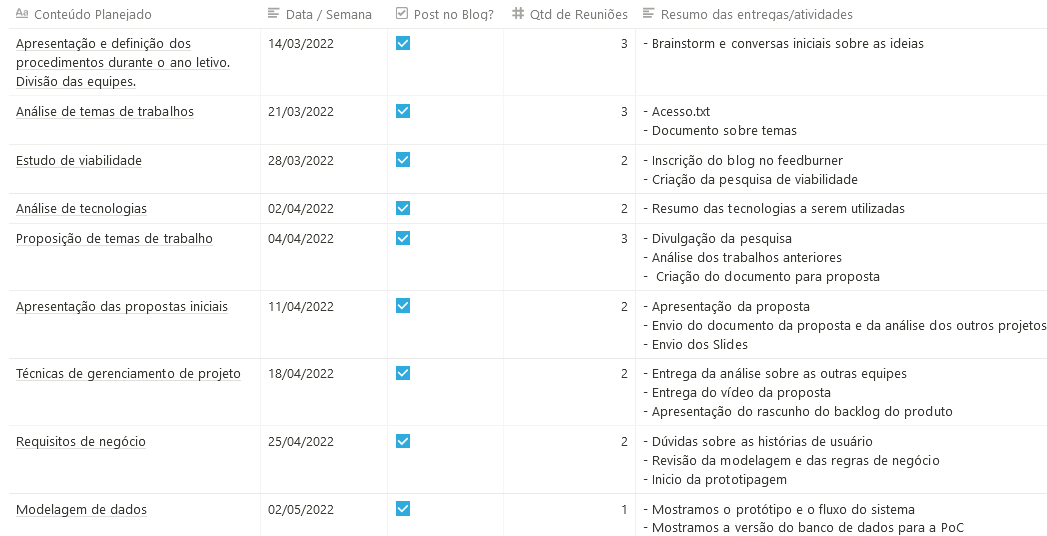
\includegraphics[width=1.0\textwidth]{anexos/Imagens_Proposta/cronograma_desenvolvimento.png}
\fonte{Os autores.}
\end{figure}
\FloatBarrier

%------------------------------------------------------------
\subsection{Artefatos e eventos utilizados}
\label{artefatos}
%------------------------------------------------------------
Tendo em vista a finalidade acadêmica do projeto, foi estipulado um valor mínimo de duas reuniões semanais dedicadas na construção, considerando a organização individual de cada membro da equipe, além da priorização para que a tomada de decisões e planejamentos sejam feitas no dia das aulas da disciplina de \acs{pds}. Sobre os artefatos e eventos do Scrum, lista-se a seguir suas funcionalidades originais, descritos por \citeonline{cruz:2018}, e como serão adaptados:

\begin{itemize}
\item \textsl{Backlog}: é descrito como uma lista de todas as características, funções, tecnologias, melhorias e correções que constituem o produto a ser entregue. É também subdividido em ``do produto'', ``da versão de entrega'' e ``da \textsl{Sprint}'';

\item \textsl{Sprint}: originalmente pensada para durar um mês ou menos e possuir uma meta estabelecida com um objetivo claro, foi pensada 
para durar até duas semanas, já que as orientações da disciplina exigem que existam entregas frequentes, isto é, todas as semanas. Portanto, o ideal é que se dê início ao trabalho a ser entregue pelo menos uma semana antes de sua entrega;

\item \textsl{Time-boxed}: é esperado que o tempo estipulado para executar uma tarefa seja cumprido e que o trabalho proposto, seja realizado. Tendo em vista os curtos prazos,
também foi adaptado conforme a entrega;

\item Planejamento da \textsl{Sprint}: ainda será utilizado para definir ``o que será feito'' e ``como'', porém, ao contrário das oito horas mínimas 
estipuladas, a equipe definiu um mínimo de duas horas para tal reunião, que poderá acontecer nas segundas-feiras, durante a aula de \acs{pds} ou aos finais de semana, logo após a finalização dos entregáveis;

\item Reuniões Diárias: não serão mantidas de maneira síncrona, visto que cada membro da equipe possui horários de disponibilidade diferentes. Porém, poderão ocorrer de forma assíncrona, de modo a compreender se existem impedimentos durante a execução das tarefas planejadas para a semana;

\item Revisão da \textsl{Sprint}: seu maior objetivo é a revisão do \textsl{Product Owner}, ou do cliente, em todos os itens concluídos pelo Time. Porém, 
não terá \textsl{Time-boxed} de quatro horas, visto que a aprovação dos professores orientadores (o cliente) pode ser mais rápida e acontecer durante a execução das tarefas. No entanto, a equipe a realizará em todo final de entrega, para que os retornos dos professores levem em consideração o trabalho final;

\item Retrospectiva da \textsl{Sprint}: possui originalmente \textsl{Time-boxed} de até três horas e é feita para identificação 
de medidas de melhoria no processo do time que serão aplicadas na próxima \textsl{Sprint}. Foi escolhido adaptá-la para acontecer às terças-feiras, antes do início das aulas, para que as entregas feitas às segundas-feiras estejam frescas e o processo realizado pelo time possa ser mais bem avaliado para a melhoria contínua.
\end{itemize}

Para a definição do \textsl{backlog} do produto, o Scrum conta com um recurso chamado histórias de usuário, que pode ser definido como: 

\begin{citacao}
História é uma descrição resumida, porém clara e objetiva, de alguma funcionalidade que deverá ser fornecida pelo produto a ser entregue, sempre do ponto de vista do usuário final. Uma história não é uma especificação completa da funcionalidade, mas uma promessa de discutir uma funcionalidade, ou, simplesmente, um lembrete de que a discussão já aconteceu. Um modelo simples de como escrever uma história seria: ``Como um <tipo de usuário>, eu quero <um objetivo> para que <atenda a uma necessidade>'' \cite{cruz:2018}.
\end{citacao}

% Entretanto, vale ressaltar que as histórias de usuário do presente projeto serão montadas somente na parte de desenvolvimento, isto é, quando o produto começar a ser construído pelo Time Scrum e após os principais itens de \textsl{backlog} estarem descritos. Como ainda se encontra na fase de planejamento e modelagem, tal recurso ainda não foi acionado no projeto.

Entretanto, vale ressaltar a respeito a utilização do \textsl{Scrum Poker} ou \textsl{Planning Poker Card}, que, segundo \citeonline{cruz:2018}, é definido como ``uma técnica que auxilia na estimativa de histórias e tarefas com base no consenso de todo o Time''. Para tanto, o Time utiliza um conjunto de cartas com valores representando os pontos ou horas por história. Sobre o funcionamento do \textsl{Planning Poker Card}:

\begin{citacao}
O seu uso é simples: o \textsl{Product Owner} ou um membro do Time apresenta a história, ou tarefa. Após uma breve discussão, cada um escolhe uma carta e a coloca virada sobre uma mesa, de forma que um não constate o valor da carta que o outro escolheu. Quando todos colocarem suas cartas, elas são desviradas para que todos vejam os valores.

Caso não haja consenso entre as cartas escolhidas, as diferenças são discutidas brevemente e uma nova rodada acontece, até que haja convergência e consenso \cite{cruz:2018}.
\end{citacao}

Para o presente projeto, o \textsl{Planning Poker Card} foi utilizado durante o processo de desenvolvimento do produto e após as histórias de usuário da \textsl{Sprint} estarem bem descritas. Vale ressaltar que este processo é apenas para estimar o trabalho da equipe e pode variar conforme o andamento do projeto.

%------------------------------------------------------------
\subsection{Métricas de Desenvolvimento}
%------------------------------------------------------------
De modo a fazer nosso processo de desenvolvimento o mais produtivo possível, e entregar o máximo do \textit{backlog} do produto, foram definidas as seguintes pontuações (\autoref{Métricas}) para identificar o grau de complexidade das tarefas de modo a priorizar o desenvolvimento daquelas que exijam um trabalho maior. Essas pontuações foram baseadas no princípio do \textit{Planning Poker Card}, no qual a pontuação das cartas usadas para a estimativa segue a sequência de \textit{Fibonacci}. 

\def\arraystretch{2}
\begin{quadro}[htb]
\centering
\ABNTEXfontereduzida
\caption{Métricas de Organização das Histórias}
\label{Métricas}
\resizebox{\linewidth}{!}{
\begin{tabular}{|c|c|p{10cm}|}
\hline
\thead{Pontuação} & \thead{Tamanho} & \thead{Descrição} \\ \hline

< 5  & Pequeno & Pontuação usada para classificar tarefas que são de nível fácil e que podem ser realizadas em um curto período. \\ \hline
5 e 8 & Médio & Pontuação usada para classificar tarefas de nível médio e exigem um desempenho maior comparada com as de nível fácil, mas não chegam a ser muito complexas. \\ \hline
$ \geq 13 $ & Grande & Pontuação usada para classificar tarefas que são de nível difícil e exigem um grande desempenho, além de precisarem de mais tempo para serem desenvolvidas. \\ \hline

\end{tabular}}\legend{Fonte: Os autores}
\end{quadro}
\FloatBarrier

Esses critérios de pontuação foram aplicados as histórias de usuário (\autoref{historias de usuario}), portanto, com o uso dessas métricas é possível priorizar tarefas mais complexas (com maior pontuação) das mais simples (com menor pontuação) além de ajudar na execução das \textsl{Sprints}. A aplicação dessas métricas pode ser constada na figura \autoref{metricas_historias}.

\begin{figure}[htb]
\centering
\caption{Histórias no Notion}
\label{metricas_historias}
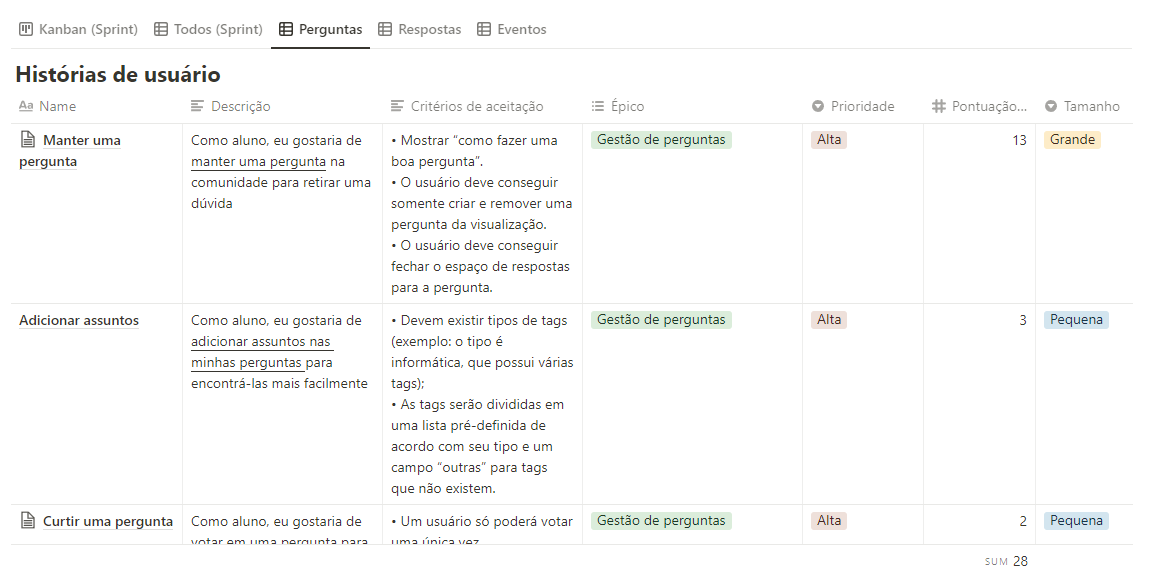
\includegraphics[width=1.0\textwidth]{anexos/Imagens_Desenvolvimento/metricas_historias.png}
\fonte{Os autores.}
\end{figure}
\FloatBarrier

A sua utilização se deu através de uma reunião realizada por todos os membros da equipe e como o auxílio do \href{https://www.scrumpoker-online.org/en/}{Scrum Poker Online} que nos forneceu as ferramentas necessárias para realizar a estimativa de pontuação.

%------------------------------------------------------------

%-------------------------------------------------------------
%------------------------------------------------------------

%------------------------------------------------------------
\section{Análise de Requisitos}
%------------------------------------------------------------
Segundo \citeonline{machado2018analise}, ao definir as características de um requisito, é preciso salientar que não são dependentes da tecnologia empregada, visto que suas especificações estão contidas no campo do cumprimento das necessidades do usuário. Dessa forma,  \citeonline{machado2018analise} define os requisitos como ``objetivos ou restrições estabelecidas por clientes e usuários do sistema que definem suas diversas propriedades''.

Assim, tanto \citeonline{machado2018analise} como \citeonline{SOMMERVILLE:2019} concordam que a fase de definição de requisitos, a chamada engenharia de requisitos, é essencial para a tomada de decisões sobre os passos para adquirir ou desenvolver o sistema. Por outro lado, Sommerville ainda acrescenta sobre a necessidade de mudança durante o desenvolvimento:

\begin{citacao}
Naturalmente, são feitas mudanças subsequentes nos requisitos de usuário, que podem ser ampliados para requisitos de sistema mais detalhados. Às vezes, pode-se utilizar uma abordagem ágil para elicitar simultaneamente os requisitos à medida que o sistema é desenvolvido, a fim de acrescentar detalhes e refinar os requisitos de usuário \cite{SOMMERVILLE:2019}.
\end{citacao}

Tendo tais definições em vista, as próximas seções visam apresentar os requisitos funcionais e não funcionais, e as regras do negócio característicos do projeto tratado neste documento. 
% Para representar os requisitos funcionais e os requisitos não funcionais se usou as histórias de usuário. Foi com base na utilização da abordagem ágil no projeto, que se definiu três prioridades principais: alta, média e baixa. 

% A prioridade alta é aquela correspondente aos requisitos obrigatórios para o funcionamento do sistema, isto é, aqueles que caso faltem, o sistema em si não existe; já na prioridade média, por exemplo, são característicos aqueles desejáveis, ou seja, são importantes para o sistema, mas não interferem diretamente numa mudança brusca de seu comportamento. Desse modo, os requisitos de prioridade baixa, são tidos como opcionais, aqueles que podem entrar no sistema eventualmente, mas que, numa fila de produção, não serão feitos antes dos demais. Vale ressaltar, por conseguinte, que tais decisões dependem da negociação entre os envolvidos no projeto e do método de produção utilizado, como descrevem \citeonline{vazquezsimoes:2016}. Os autores ainda completam, dizendo:

% \begin{citacao}
% A priorização tem como função assegurar que os recursos do projeto sejam focados nos itens mais relevantes. Daí a importância de, na especificação, diferenciar cada requisito em termos de importância, dentre dezenas ou centenas de outros requisitos.

% A responsabilidade por definir a prioridade do requisito deveria ser da parte interessada, facilitada pelo gerente de projetos \cite{vazquezsimoes:2016}.
% \end{citacao}

%------------------------------------------------------------
\subsection{Histórias de Usuário}
%------------------------------------------------------------
Segundo \citeonline{cruz:2018} as histórias de usuário se caracterizam como uma descrição resumida, clara e objetiva de uma funcionalidade fornecida pelo produto a ser entregue, visando o ponto de vista final do usuário. Ainda segundo o autor para uma história ser tida como completa, ela deve possuir uma descrição objetiva e critérios de aceitação, esses critérios representam o que ela precisa fazer para ser considerada válida.

No projeto, a equipe aproveitou as histórias de usuário para representar os requisitos funcionais e não funcionais, dessa forma os requisitos funcionais podem ser identificados a partir do nome das histórias, e o não funcionais por meio dos critérios de aceitação definidos para tais.

Todas as histórias se encontram no \autoref{historias de usuario} e apresentam sete componentes: o seu nome, a sua descrição, seus critérios de aceitação, o épico a qual pertence, a pontuação que ela recebeu no \textsl{Planning Poker Card}, a estimativa de tamanho conforme a sua pontuação e a sua prioridade conforme o seu tamanho e pontuação. Ainda com o fim de organizá-las foram separadas por meio dos seguintes épicos:

\begin{itemize}
\item {\textbf{Gestão de Perguntas:}} Para este épico foram destinadas às histórias de usuário do \autoref{resumo: gestão de perguntas}. Logo, os devidos detalhes de cada história de usuário se encontra na \autoref{gestão_perguntas} do apêndice.

\def\arraystretch{2}
\begin{quadro}[htb]
\centering
\ABNTEXfontereduzida
\caption{Resumo: Gestão de perguntas}
\label{resumo: gestão de perguntas}
\resizebox{\linewidth}{!}{
\begin{tabular}{|p{6.5cm}|c|c|c|}
\hline
\thead{História} & \thead{Pontuação} & \thead{Tamanho} & \thead{Prioridade}\\
\hline
Manter uma pergunta & 13 & Grande & ALTA \\ \hline
Filtrar perguntas & 8 & Médio & MÉDIA \\ \hline
Adicionar assuntos & 3 & Pequeno & ALTA \\ \hline
Curtir uma pergunta & 2 & Pequeno & ALTA \\ \hline
Buscar perguntas & 2 & Pequeno & MÉDIA  \\ \hline

\end{tabular}}\legend{Fonte: Os autores}
\end{quadro}
\FloatBarrier 

Como a primeira história a ser desenvolvida pela equipe se encontrava nesse épico, era necessário considerar também a configuração de ambiente, dessa forma, ele acabou recebendo uma estimava global de esforço maior, em relação aos outros, totalizando 28 pontos.

\item {\textbf{Gestão de Respostas:}} Para este épico foram destinadas às histórias de usuário do \autoref{resumo: gestão de respostas}. Logo, os devidos detalhes de cada história de usuário se encontra na \autoref{gestão_respostas} do apêndice.

\def\arraystretch{2}
\begin{quadro}[htb]
\centering
\ABNTEXfontereduzida
\caption{Resumo: Gestão de respostas}
\label{resumo: gestão de respostas}
\resizebox{\linewidth}{!}{
\begin{tabular}{|p{6.5cm}|c|c|c|}
\hline
\thead{História} & \thead{Pontuação} & \thead{Tamanho} & \thead{Prioridade}\\
\hline
Manter uma resposta & 5 & Médio & ALTA \\ \hline
Curtir uma resposta & 1 & Pequeno & ALTA \\ \hline

\end{tabular}}\legend{Fonte: Os autores}
\end{quadro}
\FloatBarrier 

Se tratando do segundo épico a ser trabalhado, a sua estimativa global de esforço foi menor em relação ao primeiro, mas nele ainda foi mantida a prioridade alta, dessa forma, o épico totalizou 6 pontos.
    
\item {\textbf{Gestão de Eventos:}} Para este épico foram destinadas às histórias de usuário do \autoref{resumo: gestão de eventos}. Logo, os devidos detalhes de cada história de usuário se encontra na \autoref{gestão_eventos} do apêndice.

\def\arraystretch{2}
\begin{quadro}[htb]
\centering
\ABNTEXfontereduzida
\caption{Resumo: Gestão de eventos}
\label{resumo: gestão de eventos}
\resizebox{\linewidth}{!}{
\begin{tabular}{|p{6.5cm}|c|c|c|}
\hline
\thead{História} & \thead{Pontuação} & \thead{Tamanho} & \thead{Prioridade}\\
\hline
Manter evento & 3 & Pequeno & BAIXA \\ \hline
Favoritar evento & 2 & Pequeno & BAIXA \\ \hline

\end{tabular}}\legend{Fonte: Os autores}
\end{quadro}
\FloatBarrier 

O épico totalizou 5 pontos, e suas histórias foram classificadas com tamanho pequeno devido à semelhança no desenvolvimento das histórias anteriores, dessa forma, foram denotadas como histórias de usuário nível fácil.

\item {\textbf{Gestão de Usuários:}} Para este épico foi destinada à história de usuário do \autoref{resumo: gestão de usuários}. Logo, seus devidos detalhes se encontra na \autoref{gestão_usuario} do apêndice.

\def\arraystretch{2}
\begin{quadro}[htb]
\centering
\ABNTEXfontereduzida
\caption{Resumo: Gestão de usuários}
\label{resumo: gestão de usuários}
\resizebox{\linewidth}{!}{
\begin{tabular}{|p{6.5cm}|c|c|c|}
\hline
\thead{História} & \thead{Pontuação} & \thead{Tamanho} & \thead{Prioridade}\\
\hline
Autenticação do usuário & 5 & Médio & ALTA \\ \hline

\end{tabular}}\legend{Fonte: Os autores}
\end{quadro}
\FloatBarrier 

O épico é responsável pelo quesito de autenticação do sistema, no entanto, por não ser uma tarefa muito complexa totalizou 5 pontos como estimativa de esforço.

\item {\textbf{Usabilidade:}} Para este épico foi destinada à história de usuário do \autoref{resumo: usabilidade}. Logo, seus devidos detalhes se encontra na \autoref{gestão_usabilidade} do apêndice.

\def\arraystretch{2}
\begin{quadro}[htb]
\centering
\ABNTEXfontereduzida
\caption{Resumo: Usabilidade}
\label{resumo: usabilidade}
\resizebox{\linewidth}{!}{
\begin{tabular}{|p{6.5cm}|c|c|c|}
\hline
\thead{História} & \thead{Pontuação} & \thead{Tamanho} & \thead{Prioridade}\\
\hline
Internacionalização & 5 & Médio & ALTA \\ \hline

\end{tabular}}\legend{Fonte: Os autores}
\end{quadro}
\FloatBarrier 

O épico é responsável para classificar entregas relacionadas a usabilidade do sistema, sendo a única mapeada até o momento, criada para a entrega do valor de disponibilidade de tradução dos conteúdos em português e inglês. Logo, o épico totalizou 5 pontos como estimativa de esforço.

\end{itemize}

%------------------------------------------------------------
\subsection{Regras de Negócio}
%------------------------------------------------------------
Regras de negócio são requisitos de domínio de aplicação tratado no desenvolvimento de um sistema, isso significa, as declarações sobre como determinada empresa faz negócio. É a partir dessas regras que se define como o negócio funciona e quais são suas especificações, além da sua importância para o desenvolvimento de um sistema, pois, auxiliam no controle dos processos, ajudam na tomada de decisões além de afetarem diretamente os requisitos funcionais, como descrevem \citeonline{dallavalle2000regras}. Dessa forma, o \autoref{regras negocio} lista as regras de negócio levantadas para o projeto \gls{ifriends}.

\def\arraystretch{2}
\begin{quadro}[thb]
\centering
\ABNTEXfontereduzida
\caption{Regras de Negócio}
\label{regras negocio}
\resizebox{\linewidth}{!}{
\begin{tabular}{|c|p{13cm}|}
\hline
\textbf{ID} & \textbf{Descrição} \\
\hline
\acs{RN}01 & Não serão permitidos usuários com os mesmos dados, ou seja, o sistema só permitirá a criação de uma conta por usuário \\
\hline
\acs{RN}02 & A fim de garantir a segurança de nossos usuários, o sistema deverá fazer uso de algumas diretrizes da Lei Marco Civil da Internet, lei n\textdegree 12.965/2014, que tem como objetivo estabelecer princípios, garantias, direitos e deveres para o uso da internet no Brasil. \\
\hline
\acs{RN}03 & Dentro do direito a exclusão, ao excluir seu perfil, o usuário deve ter ciência de que suas perguntas e respostas serão mantidas na comunidade, porém como parte de um usuário anônimo (exemplo: user12345678). \\
\hline
\acs{RN}04 & O usuário deve levar em consideração as boas prática para o desenvolvimento de uma pergunta (\autoref{boa-pergunta}).  \\
\hline

\end{tabular}}\legend {Fonte: os autores}
\end{quadro}
\FloatBarrier 

%------------------------------------------------------------
\subsection{Partes interessadas e usuários}
%------------------------------------------------------------
Segundo \citeonline{BibEntry2021Nov} por \textit{stakeholders} ou partes interessadas se entende todas as organizações ou grupo de pessoas que possam apresentar interesse ou serem afetadas pelas ações de uma determinada empresa. Nas partes interessadas podem se classificar desde colaboradores, tidos como \textit{stakeholders} internos, até fornecedores, investidores, clientes e comunidades, tidos como externos. 

Dessa forma, no \autoref{Partes interessadas} foram representados os \textit{stakeholders} considerados para o desenvolvimento do projeto \gls{ifriends}.

\def\arraystretch{2}
\begin{quadro}[htb]
\centering
\ABNTEXfontereduzida
\caption{Partes interessadas}
\label{Partes interessadas}
\resizebox{\linewidth}{!}{
\begin{tabular}{|c|c|p{9cm}|}
\hline
\thead{Nome} & \thead{Nível de influência} & \thead{Interesses e Expectativas}\\
\hline
Discentes & Alto & Participar do fórum de perguntas e respostas, assim como gerenciar os eventos \\ \hline
Docentes & Médio & Acompanhamento extracurricular das dificuldades relacionadas a respeito do conteúdo lecionado. \\ \hline
Coordenação e Direção & Médio & Regulação no uso adequado do sistema, ou seja, se ele esta cumprindo o que foi planejado inicialmente. \\ \hline
Pais e responsáveis & Médio & Estar a par dos meios extracurriculares aderidos pela instituição. \\ \hline

\end{tabular}}\legend{Fonte: Os autores}
\end{quadro}
\FloatBarrier 

Já por usuário, segundo \citeonline{BibEntry2017Oct}, são caracterizados aqueles que usam um determinado sistema, não sendo necessário um conhecimento técnico completo para compreender e executá-lo. Dessa forma, o \autoref{usuários} apresenta todos os possíveis usuários que possam ter acesso ao projeto de sistemas \gls{ifriends}.

\def\arraystretch{2}
\begin{quadro}[htb]
\centering
\ABNTEXfontereduzida
\caption{Usuários}
\label{usuários}
\resizebox{\linewidth}{!}{
\begin{tabular}{|c|p{5cm}|p{7cm}|}
\hline
\thead{Nome} & \thead{Descrição} & \thead{Ações} \\
\hline
\glspl{friend} & Dicentes que tenham interesse no fórum e nos eventos. & Este tipo de usuário pode visualizar, respoder, curtir, denunciar, cadastrar perguntas e respostas no fórum além de poder realizar as mesmas ações na seção de eventos. \\ 
\hline
Docentes & Professores que tenham interesse em realizar acompanhamento de seus alunos por meio do \gls{ifriends}. & Este tipo de usuário possui as mesmas ações que o tipo de usuário \glspl{friend}. \\ 
\hline
Usuários externos & Pessoas que desejem conhecer a comunidade e que não façam parte da instituição. & Este tipo de usuário terá apenas a possibilidade de visualizar páginas públicas. \\
\hline

\end{tabular}}\legend{Fonte: Os autores}
\end{quadro}
\FloatBarrier 

O termo \glspl{friend} surge devido a um apelido destinado aos usuários do sistema \gls{ifriends}, além de ele nos ajudar a demostrar melhor as funcionalidades do sistema, o mesmo também nos permite demostrar a importância e o carinho desempenhado pela equipe na produção deste projeto.  

%------------------------------------------------------------
%-------------------------------------------------------------
\section{Modelagem}
%-------------------------------------------------------------
Segundo \citeonline{SOMMERVILLE:2019}, a modelagem de sistemas é definida como ``um processo de desenvolvimento de modelos abstratos de um sistema, cada um apresentando uma visão diferente do mesmo''. Para isso, descreve também que são geralmente usadas notações gráficas baseadas nos tipos de diagrama em \acs{uml} durante o processo de engenharia de requisitos ``para ajudar a derivar os requisitos detalhados de um sistema; durante o processo [...]; e depois da implementação, para documentar a estrutura e operação do sistema'' \cite{SOMMERVILLE:2019}. 

%-------------------------------------------------------------
\subsection{Diagrama de Casos de Uso}
%-------------------------------------------------------------
De acordo com \citeonline{umlGuedes}, o diagrama de casos de uso \acs{uml} é descrito como:

\begin{citacao}
O diagrama de casos de uso [...] tem por objetivo apresentar uma visão externa geral das funcionalidades que o sistema deverá oferecer aos usuários, sem se preocupar com a questão de como tais funcionalidades serão implementadas. [...] É de grande auxílio para a identificação e compreensão dos requisitos do sistema, ajudando a especificar, visualizar e documentar as características, funções e serviços do sistema desejados pelo usuário \cite{umlGuedes}.
\end{citacao}

Logo, a \autoref{diagrama_CasosUso} representa os casos de uso do projeto de sistema \gls{ifriends}.

\begin{figure}[htb]
\centering
\caption{Diagrama de Casos de Uso}
\label{diagrama_CasosUso}
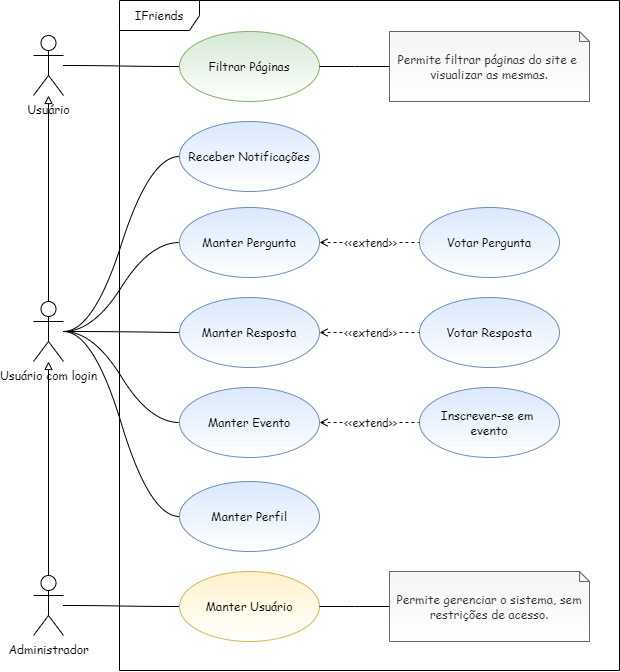
\includegraphics[width=1.0\textwidth]{anexos/Imagens_Diagramas/CasosDeUso_IFriends.png}
\fonte{Os autores.}
\end{figure}
\FloatBarrier

%-------------------------------------------------------------
\subsection{Diagrama de Classes}
%-------------------------------------------------------------
Segundo \citeonline{SOMMERVILLE:2019} os diagramas de classe são usados no desenvolvimento de um sistema orientado a objetos para realizar a demonstração das classes e suas associações entre elas. O autor ainda complementa com a seguinte ideia geral: 

\begin{citacao}
De maneira geral, uma classe pode ser encarada como uma definição geral de um tipo de objeto de sistema. Uma associação é um vínculo entre classes, que indica a existência de um relacionamento entre elas. Consequentemente, cada classe pode precisar de alguns conhecimentos a respeito de sua classe associada \cite{SOMMERVILLE:2019}. 
\end{citacao}

Dessa forma, a \autoref{Entidades DdC} representa as entidades do diagrama de Classes do projeto \gls{ifriends}.

% Entidades
\begin{figure}[htb]
\centering
\caption{Diagrama de Classes}
\label{Entidades DdC}
\includesvg[inkscapelatex=false,width=1\textwidth]{anexos/Imagens_Diagramas/Entidades_DiagramaClasses.svg}
\fonte{Os autores.}
\end{figure}
\FloatBarrier

Já a \autoref{Services DdC} representa as classes de serviço e seus respectivos métodos dentro da \gls{api} \gls{ifriends}.

% Services
\begin{figure}[htb]
\centering
\caption{Diagrama de Classes}
\label{Services DdC}
\includesvg[inkscapelatex=false,width=1\textwidth]{anexos/Imagens_Diagramas/Services_DiagramaClasses.svg}
\fonte{Os autores.}
\end{figure}
\FloatBarrier

%-------------------------------------------------------------
\subsection{Diagrama de Entidade e Relacionamento}
%-------------------------------------------------------------
De acordo com \citeonline{leal2015linguagem}, a abordagem entidade-relacionamento é a técnica de modelagem de dados mais difundida e utilizada e representa um modelo conceitual do banco de dados. Nela, a estrutura do banco de dados é descrita como coleção de entidades, relacionamentos e representada graficamente por meio do Diagrama Entidade Relacionamento.

Através dele, é possível descrever um subconjunto do mundo real que será retratado no banco de dados com um alto nível de abstração. Além disso, o modelo Entidade Relacionamento é um modelo formal e caracteriza-se por ter uma grande capacidade semântica, o que garante que todos possam ter o mesmo entendimento \cite{leal2015linguagem}.

A \autoref{diagrama_EntidadeRelacionamento} representa o \ac{der} do projeto de sistema \gls{ifriends}.

\begin{figure}[htb]
\centering
\caption{Diagrama de Entidade e Relacionamento}
\label{diagrama_EntidadeRelacionamento}
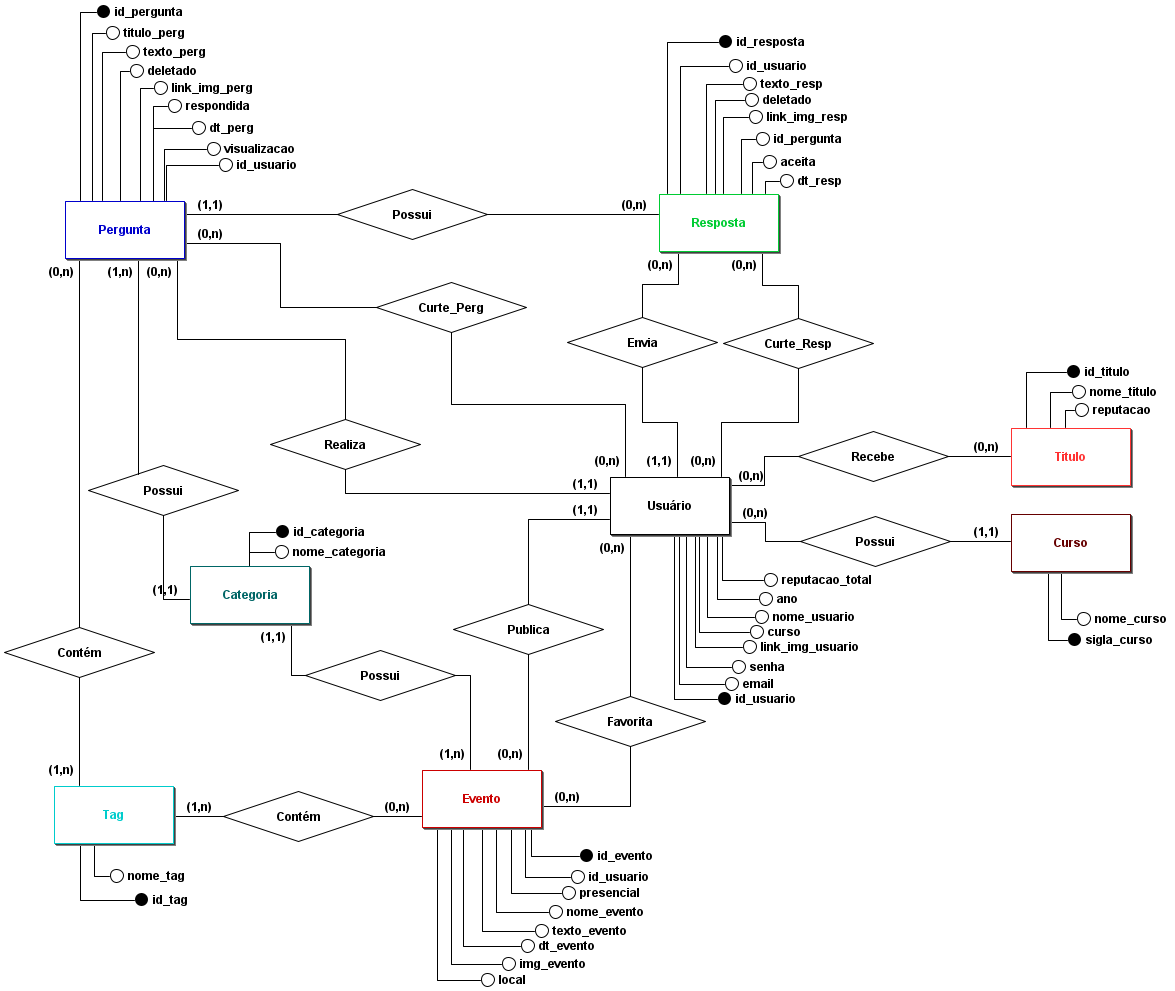
\includegraphics[width=1\textwidth]{anexos/Imagens_Diagramas/DER_IFriends.png}
\fonte{Os autores.}
\end{figure}
\FloatBarrier

%-------------------------------------------------------------
\subsection{Diagrama de Tabelas Relacionais}
%-------------------------------------------------------------
O Diagrama de Tabelas Relacionais \acs{dtr} representa o modelo lógico do Banco de Dados. Segundo \citeonline{utilidadepublica:201?}, através do modelo lógico é representado de maneira mais clara as entidades e os relacionamentos, pois considera algumas limitações e implementa recursos como adequação de padrão e nomenclatura, define as chaves primárias e estrangeiras, normalização, integridade referencial, entre outras.

Deste modo, a \autoref{diagrama_TabelasRelacionais} representa o \ac{dtr} do projeto de sistema \gls{ifriends}.

\begin{figure}[htb]
\centering
\caption{Diagrama de Tabelas Relacionais}
\label{diagrama_TabelasRelacionais}
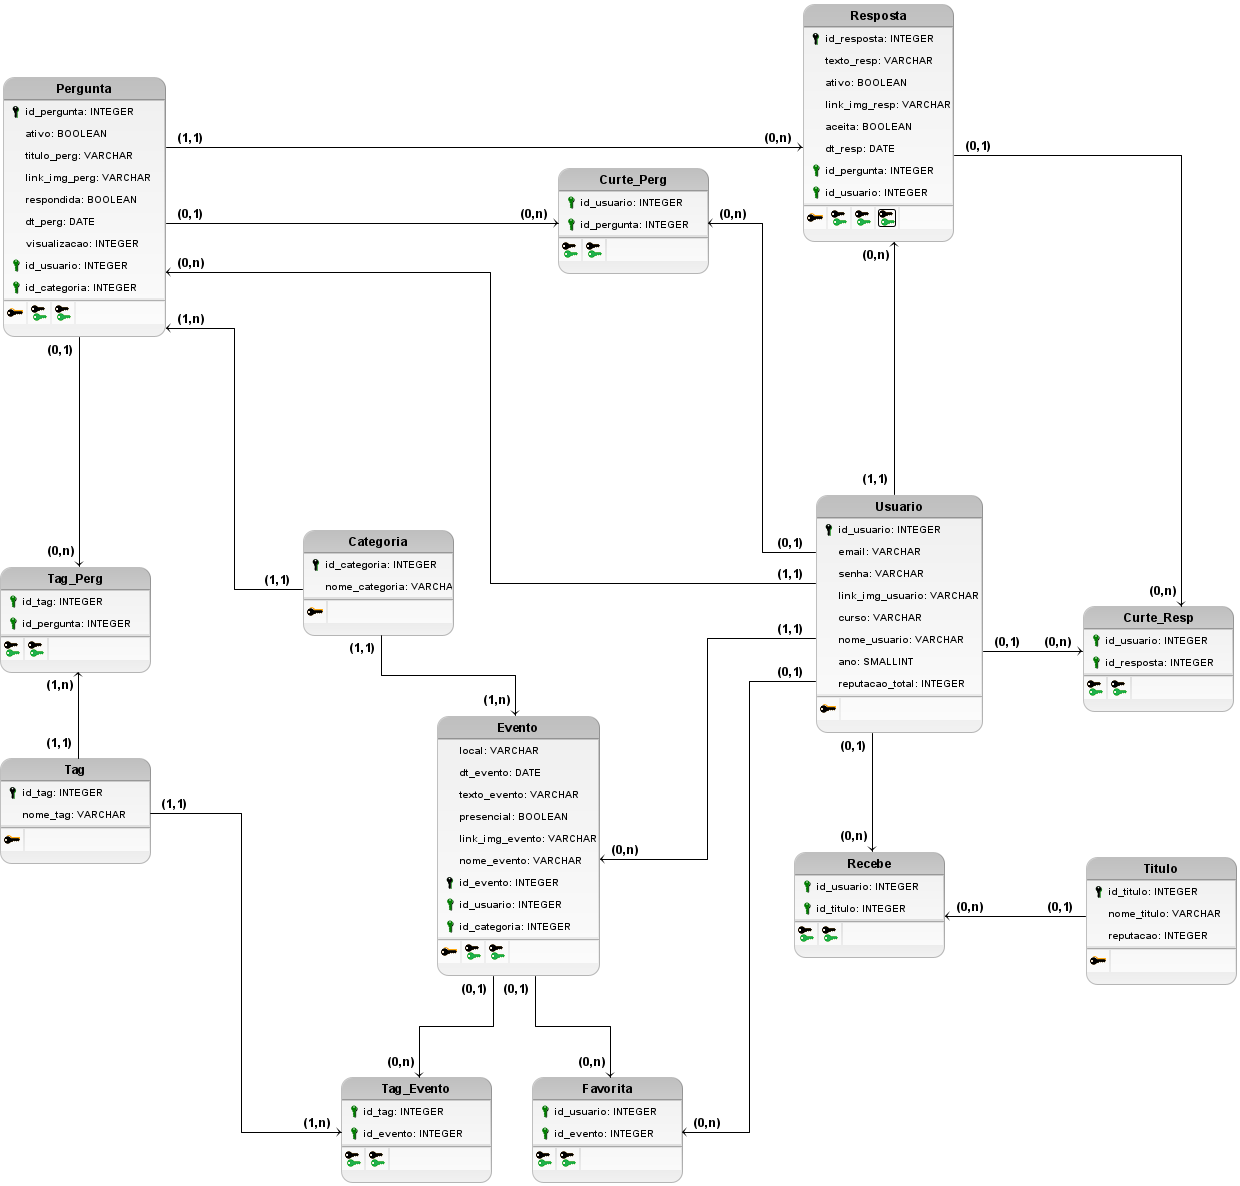
\includegraphics[width=1\textwidth]{anexos/Imagens_Diagramas/DTR_IFriends.png}
\fonte{Os autores.}
\end{figure}
\FloatBarrier

%-------------------------------------------------------------
\subsection{Dicionário de Dados}
%-------------------------------------------------------------
O \ac{dd} é responsável por armazenar as informações de configuração do banco de dados e as estruturas que compõem suas respectivas tabelas. As estruturas definem os campos e suas propriedades \cite{alvesbanco}.

Conforme \citeonline{date2004introdução}, o \ac{dd} é o lugar em que, dentre outras coisas, todos os diversos esquemas (externo, conceitual, interno) e todos os mapeamentos correspondentes são mantidos.

O \ac{dd} contém os metadados, dados que explicam dados, com relação aos diversos objetos que são de interesse do próprio sistema. Exemplos desses objetos incluem índices, usuários, restrições de integridade, restrições de segurança, e assim por diante, informações que essenciais para que o sistema faça seu trabalho apropriadamente \cite{date2004introdução}.

De tal modo, no \autoref{dicionario de dados} encontram-se os quadros que representam o \ac{dd} das tabelas de banco de dados do projeto \gls{ifriends}.

%------------------------------------------------------------

%------------------------------------------------------------
%--------------------------------------------------------------
\section{Design do projeto}
%--------------------------------------------------------------
Cogitando a missão do projeto, surgiu a ideia de dar o nome \gls{ifriends} para o sistema, cuja origem é a junção de duas palavras: IF e \textsl{friends}. Isto devido a elas retratarem bem o âmbito que será atingido, já que tais palavras em conjunto transmitem o significado de ``amigos do \acs{ifsp}'', nome ideal para um projeto que visa tornar a interação dos alunos mais favorável.

A próxima etapa do desenvolvimento inicial da marca foi a elaboração de uma logo, assim como a definição das cores iniciais do sistema. A logo foi desenvolvida por meio do \gls{canva}, pois a plataforma se encontrava nos intermédios necessários para a elaboração da mesma. 

\begin{figure}[htb]
\centering
\caption{Logo do projeto}

\includegraphics[width=0.3\textwidth]{anexos/Imagens_Proposta/logo.png}
\fonte{Os autores}
\end{figure}
\FloatBarrier

Já a seleção das cores iniciais do sistema traçou um caminho através de um estudo a respeito da psicologia das cores, visto que a equipe se preocupou em passar uma boa experiência até mesmo no quesito visual. Dessa forma, se definiu o azul e suas variações como a cor principal do sistema, já que segundo \citeonline{Tornos2021Sep}, os tons de azul se associam a princípios como: proteção, tranquilidade, fidelidade, compromisso, verdade, estabilidade, criatividade, entre outros. Vale ressaltar que o sistema ainda contará com outras cores, como roxo e algumas de suas variações, cores de sistema: variações de verde e vermelho, e cores neutras: variações de preto, cinza e branco.

Ainda, outro ponto considerado na criação da proposta foi a experiência do usuário final, pois mostrado assim como na \autoref{pesquisa}, a equipe se preocupou em estudar e conhecer melhor as dores deles. Visto que, segundo \citeonline{BibEntry2020Aug}, para tornar essa experiência agradável o sistema deve recorrer aos requisitos do modelo de colmeia desenvolvido por Peter Morville, sendo eles: útil, utilizável, desejável, acessível, confiável, localizável e valioso, conforme observado na \autoref{modelo colmeia}.

\begin{figure}[htb]
\centering
\caption{\label{modelo colmeia} Modelo Colmeia}
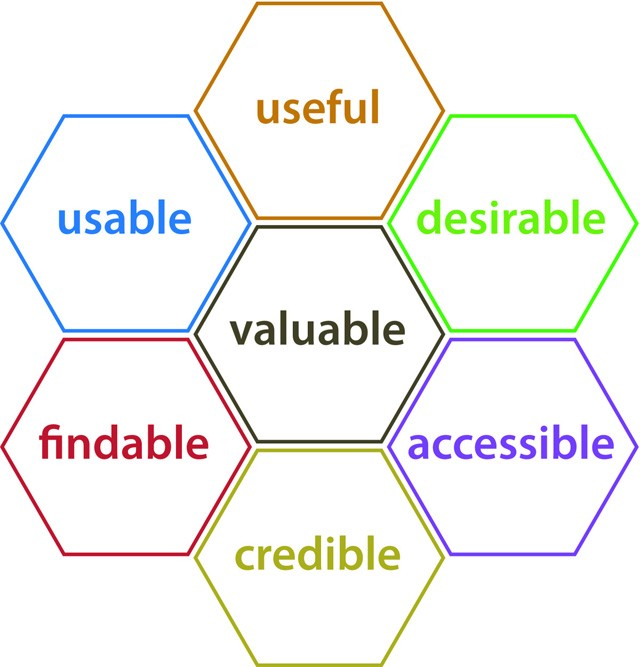
\includegraphics[width=0.3\textwidth]{anexos/Imagens_Proposta/modelo_colmeia.jpg}
\fonte{liferay.com}
\end{figure}
\FloatBarrier

% -------------------------------------------------------------
\subsection{Prototipagem}
% -------------------------------------------------------------
Para a prototipação se considerou os apontamentos de \citeonline{ferreira:2020} qual considera que ``prototipar é trazer, para o mundo real, o mundo palpável, as ideias de negócio construídas no mundo abstrato, na teoria''. Isto é, o autor comenta que um protótipo é um recurso utilizado para demonstrar e escolher a solução para representar uma ideia, podendo ser efetuado com entregas digitais, como telas de sistema. Dado isto, a próxima seção apresentará as telas prototipadas do projeto de sistema \gls{ifriends}.

Ainda, para auxiliar na prototipação das telas, foi elaborado um mapa mental de modo a representar melhor o fluxo do nosso projeto, que pode ser conferido na \autoref{Fluxo da aplicação}.

\begin{figure}[htb]
\centering
\caption{\label{Fluxo da aplicação} Fluxo da aplicação}
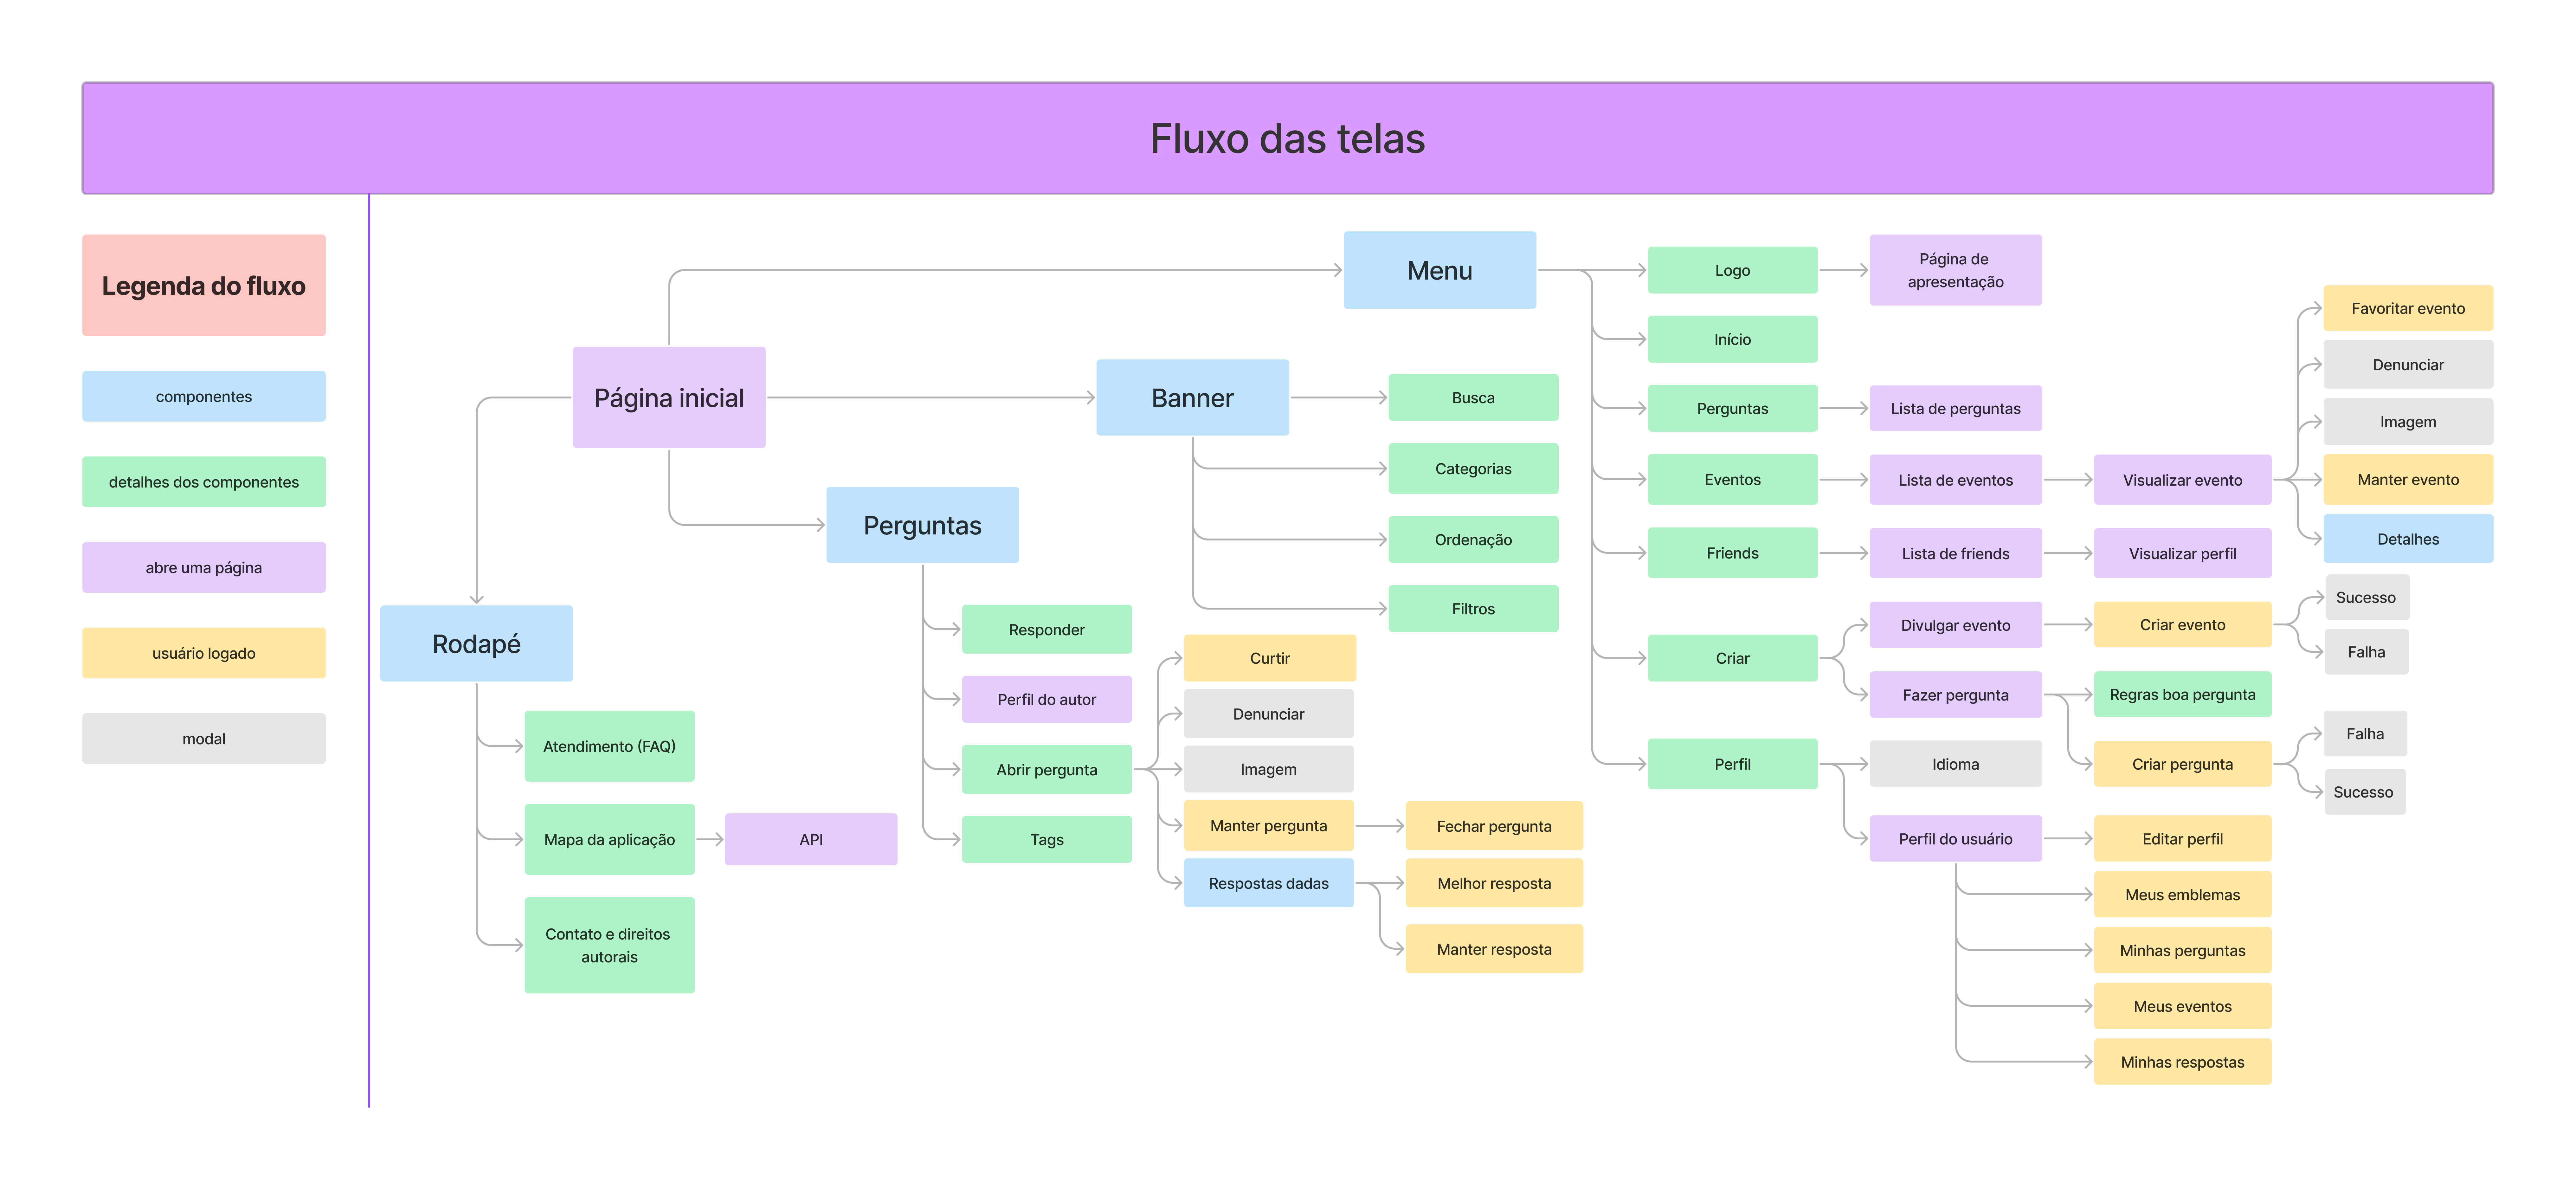
\includegraphics[width=1\textwidth]{anexos/Imagens_Prototipo/fluxo_telas.png}
\fonte{Os autores}
\end{figure}
\FloatBarrier

% -------------------------------------------------------------
\subsubsection{Protótipos de alta fidelidade}
% -------------------------------------------------------------
As figuras referentes a prototipagem de alta fidelidade podem ser encontradas no \autoref{prototipação}, onde cada tela apresenta uma breve contextualização sobre o seu conteúdo. De todo modo, a apresentação pode ser visualizada também pelo \href{https://www.figma.com/proto/GhIlybDubGmr3NkRU0a9GP/Protótipo---IFriends?node-id=73\%3A321}{Figma}.

%------------------------------------------------------------

%------------------------------------------------------------
%--------------------------------------------------------------
\section{Swagger na API}
%--------------------------------------------------------------
O Swagger, de acordo com sua documentação, é um \gls{framework} de código aberto que possui ferramentas que auxiliam na documentação dos serviços de uma \gls{REST API} com especificação \gls{openAPI}, o sistema deve apenas conter protocolos \acs{http} para aplica-lo, independente da linguagem que está sendo utilizada. O Swagger realiza a descrição de todos os recursos da \acs{api}, mostrando quais métodos \acs{http}, entidades, operações possíveis e parâmetros a serem enviados de cada \glspl{endpoint} da \gls{REST API}, por uma interface que a tecnologia disponibiliza, o Swagger UI. Portanto, este \gls{framework} facilita o entendimento do usuário em relação aos serviços de uma \acs{api}, proporcionando produtividade ao desenvolvedor.

Para a \acs{api} do projeto, está sendo utilizado a versão 3 do Swagger, pois esta versão é a mais atual e exige menos linhas de código para implementa-la, além de nos dar mais recursos, principalmente em relação à autenticidade do sistema, segundo sua documentação. O Swagger foi implementado em um arquivo dependências gerenciado pelo \gls{Maven}, após isso foi ajustada através de uma classe de configuração do \gls{SpringBoot} para geração do documento \gls{openAPI} do sistema. A \autoref{swagger API} mostra a interface do Swagger UI da \acs{api} que está sendo desenvolvida.

\begin{figure}[htb]
\centering
\caption{\label{swagger API} Swagger UI da API}
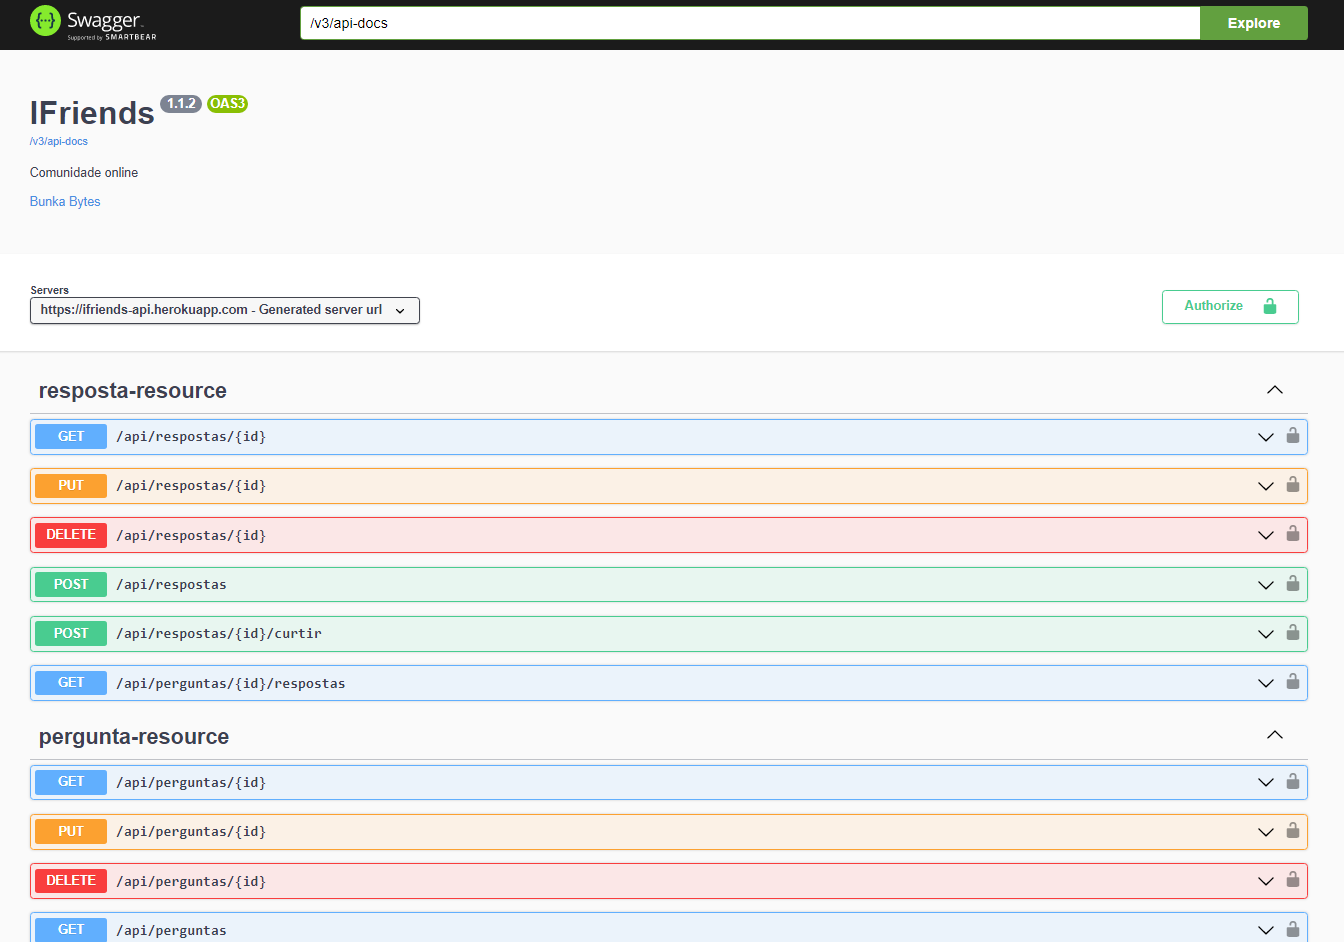
\includegraphics[width=1\textwidth]{anexos/Imagens_Swagger/API_swagger.png}
\fonte{os autores}
\end{figure}
\FloatBarrier

Como foi possível constatar na \autoref{swagger API}, no canto superior da interface indica informações gerais do projeto como o nome da \acs{api}, versão, descrição e nome da equipe. Já a parte inferior é mostrado o nome da classe de controle e a URI de cada requisição com seus métodos \acs{http}. O botão \textit{``Authorize''} é a principal função, pois este nos permite colocar o \acs{jwt} para verificar o usuário que está realizando a requisição. Após abrir um terminal, é apresentado os parâmetros, o corpo da requisição e a descrição da resposta com o código de estado, como é possível observar na \autoref{demostracao swagger API}.

\begin{figure}[htb]
\centering
\caption{\label{demostracao swagger API} Exemplo Swagger na API}
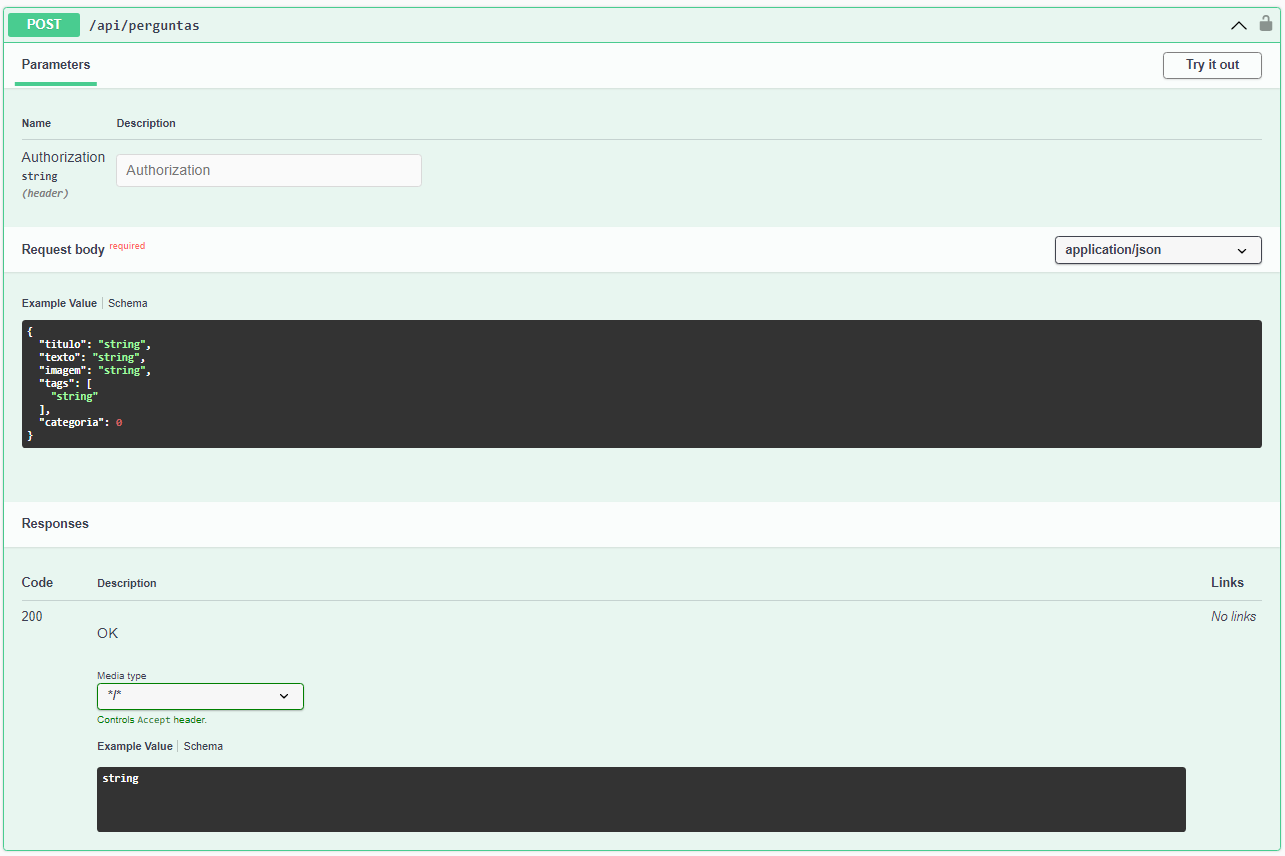
\includegraphics[width=1\textwidth]{anexos/Imagens_Swagger/API_swagger_demostracao.png}
\fonte{os autores}
\end{figure}
\FloatBarrier

%------------------------------------------------------------

%------------------------------------------------------------
%--------------------------------------------------------------
\section{Análise de segurança}
%--------------------------------------------------------------
Para a análise de segurança das aplicações, cada qual publicada no \gls{heroku} e no \gls{vercel}, através de suas URLs próprias (ifriends-api e ifriends, respectivamente), foi feita uma análise pelo \href{https://www.ssllabs.com/}{SSL Labs}, visto que o \gls{heroku} utiliza um certificado básico com suporte para \acs{tls} 1.2 e \acs{hsts}, já que o suporte completo com o \acs{acme} na comunicação via \href{https://letsencrypt.org/getting-started/}{\textsl{Let's Encrypt}} e adição de certificados manuais, o \gls{heroku} só os disponibiliza \href{https://devcenter.heroku.com/articles/ssl}{ em versões pagas}. O \acs{vercel}, por outro lado, possui suporte completo para integração com o \acs{acme}, conforme descrito em sua \href{https://vercel.com/blog/automatic-ssl-with-vercel-lets-encrypt}{documentação oficial}.

De todo modo, é possível observar que ambas as aplicações receberam a nota mínima estipulada, conforme demonstrado na \autoref{analise_ssllabs_api_heroku} e na \autoref{analise_ssllabs_frontend_heroku}.

\begin{figure}[htb]
\centering
\caption{\label{analise_ssllabs_api_heroku} Análise de segurança na API}
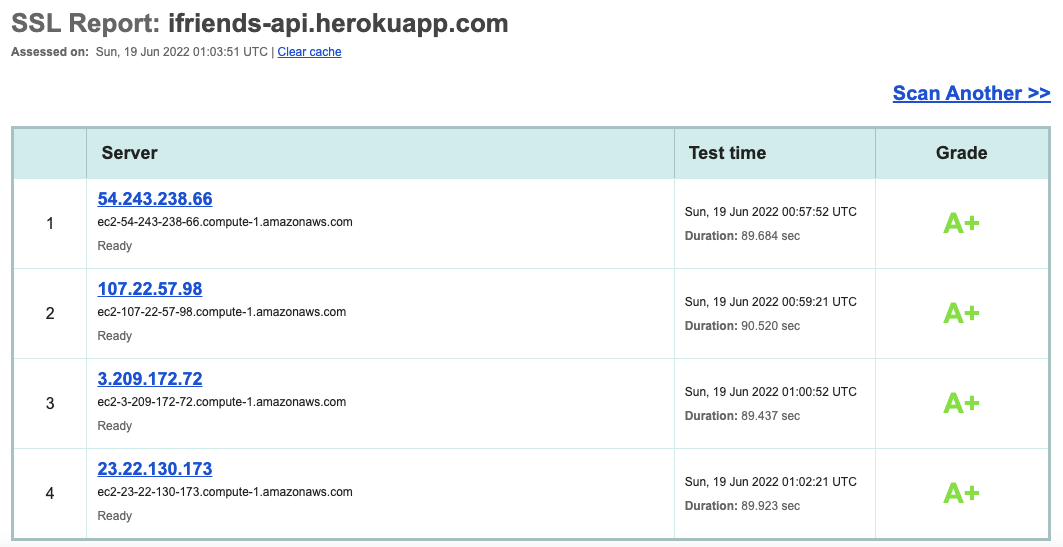
\includegraphics[width=1\textwidth]{anexos/Imagens_Seguranca/analise_ssllabs_api_heroku.png}
\fonte{Os autores}
\end{figure}
\FloatBarrier
A análise completa do que está descrito na \autoref{analise_ssllabs_api_heroku} também se encontra disponível para visualização \href{https://www.ssllabs.com/ssltest/analyze.html?d=ifriends-api.herokuapp.com}{aqui}.

\begin{figure}[htb]
\centering
\caption{\label{analise_ssllabs_frontend_heroku} Análise de segurança no Front-end}
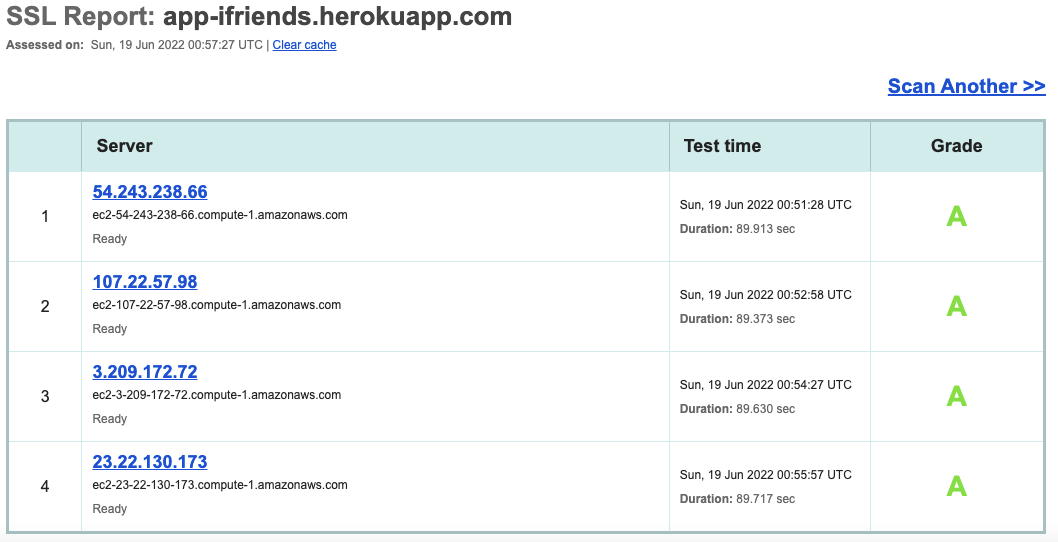
\includegraphics[width=1\textwidth]{anexos/Imagens_Seguranca/analise_ssllabs_frontend_heroku.png}
\fonte{Os autores}
\end{figure}
\FloatBarrier

A análise completa do que está descrito na  \autoref{analise_ssllabs_frontend_heroku} também se encontra disponível para visualização \href{https://www.ssllabs.com/ssltest/analyze.html?d=ifriends.vercel.app}{aqui}.

Além disso, conforme os requisitos da disciplina, a \acs{api} teve suas respostas \acs{http} analisadas pelo \href{https://securityheaders.io}{\textit{Security Headers}}, e conforme observado na \autoref{analise_http_response_api}, a aplicação conseguiu configurar todos os cabeçalhos básicos de segurança requeridos na análise.

\begin{figure}[htb]
\centering
\caption{\label{analise_http_response_api} Análise de respostas HTTP na API}
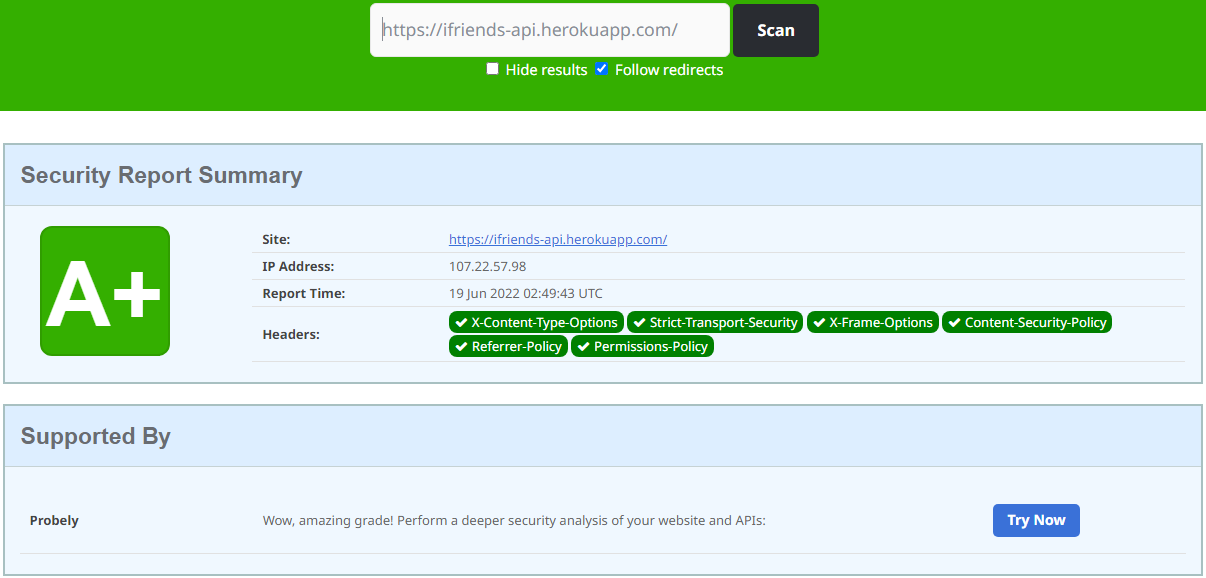
\includegraphics[width=1\textwidth]{anexos/Imagens_Seguranca/analise_http_response_api.png}
\fonte{Os autores}
\end{figure}
\FloatBarrier

Foi escolhido e aplicado pela equipe o \gls{vercel} como principal servidor de hospedagem para o lado do cliente, visto que ele possui todos os requisitos de segurança exigidos pela disciplina, assim como o certificado de \acs{dns} e suporte completo ao \acs{tls} de forma gratuita. Já para o servidor, sua hospedagem foi mantida no \gls{heroku} pela facilidade que ele oferece em hospedar o sistema juntamente com \acs{sgbd} já nativo do servidor, além de ser gratuito e ainda possuir barreiras mínimas de segurança.

\section{Análise estática de código}

De acordo com \citeonline{teixeira2007avaliaccao}, a análise estática tem como objetivo diminuir o impacto dos erros originados pelos próprios programadores sobre um determinado sistema/programa, conforme explica:

\begin{citacao}
As ferramentas de análise estática facilitam a detecção de anomalias ou erros de codificação existentes numa aplicação. Estas ferramentas vêm ajudar a eliminar lapsos cometidos
pelos programadores, podendo ter um impacto significativo no ciclo de desenvolvimento de
um produto, permitindo poupar tempo e dinheiro \cite{teixeira2007avaliaccao}.
\end{citacao}

Levando em conta os apontamentos feitos pelo autor, esta seção está reservada para algumas análises estáticas feitas sobre os códigos do \gls{ifriends} até o momento.

Foi utilizado o validador \textsl{FindBugs} como analisador estático do código feito em Java, isto é, da parte \gls{back-end} do sistema. O \textsl{FindBugs} possui uma integração amigável com o \gls{Eclipse}, facilitando a sua instalação no projeto \textsl{Spring Boot} desenvolvido atualmente. Além disso, o programa possui vários critérios de análise e classificações para os erros, deixando claros os riscos, caso passem despercebidos. A \autoref{relatorio analise estatica} mostra todos os pacotes e classes, assim como a quantidade de erros encontrados e outras informações sobre o projeto.

\begin{figure}[htb]
\centering
\caption{\label{relatorio analise estatica} Relatório do FindBugs}
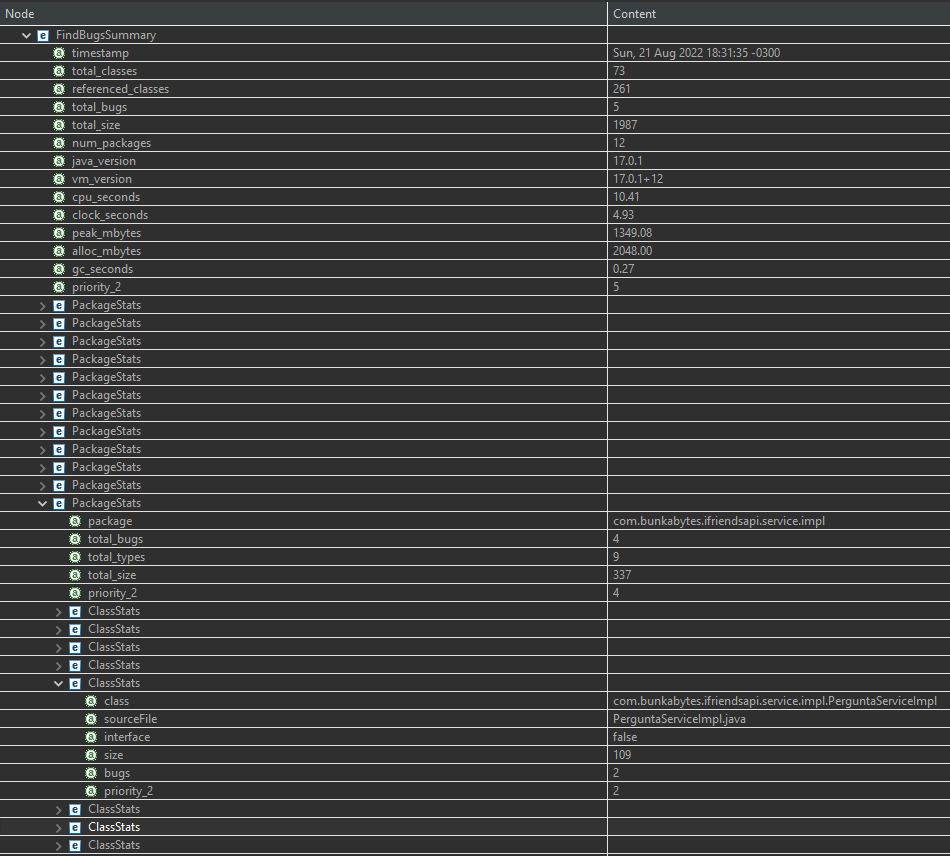
\includegraphics[width=1\textwidth]{anexos/Imagens_AnaliseEstatica/relatorio-findbugs.png}
\fonte{Os autores}
\end{figure}
\FloatBarrier


%------------------------------------------------------------

%------------------------------------------------------------
%--------------------------------------------------------------
\section{Métricas do projeto}
% ------------------------------------------------------------
Visando acompanhar quantitativamente a evolução no desenvolvimento do \gls{ifriends}, a equipe realiza medições mensalmente, que podem ser observadas na \autoref{tabela de métricas}, conforme os itens: arquivos, classes, porcentagem da cobertura dos testes unitários, \textit{commits}, entidades alocadas no banco de dados, interfaces, quantidade de linhas de código, métodos, \textit{posts} do \textit{blog}, quantidade de testes unitários aplicados, requisitos cumpridos, quantidade de reuniões, tamanho da aplicação em \textit{Mega Bytes} e vídeos publicados no canal do \gls{youtube}. Vale lembrar que os valores inseridos serão contados de forma acumulativa. 

\begin{figure}[htb]
\centering
\caption{Tabela de métricas}
\label{tabela de métricas}
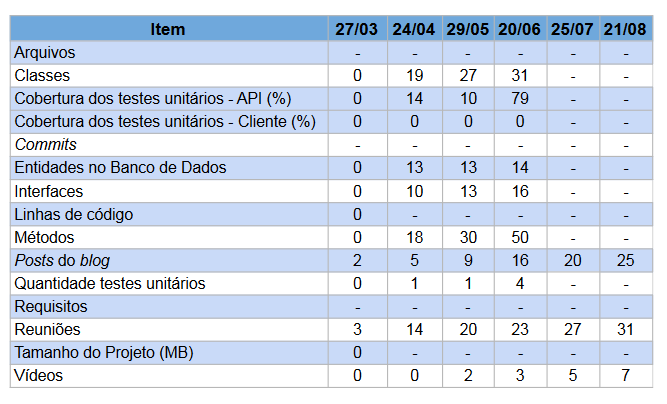
\includegraphics[width=1.0\textwidth]{anexos/Imagens_PesquisaAceitacao/Metricas.png}
\fonte{Os autores}
\end{figure}
\FloatBarrier
% ------------------------------------------------------------
\section{Plano de testes}
%--------------------------------------------------------------
Segundo \citeonline{Polo:2020}, por definição, os testes de \textit{software} visam assegurar que um sistema/programa atenda às necessidades dos seus usuários, assim como também permitem descobrir defeitos no funcionamento antes de disponibilizá-lo para uso. Na realização dos testes, segundo \citeonline{SOMMERVILLE:2019}, são usados dados artificiais para a sua execução.

\begin{citacao}
Os resultados dos testes são verificados para descoberta de erros, anomalias ou informações não funcionais sobre a sua execução, por exemplo, análise de desempenho, utilização de memória etc \cite{Polo:2020}.
\end{citacao}

Considerando os apontamentos dos autores, e de modo a garantir um bom funcionamento do sistema \gls{ifriends} além de prevenir eventuais erros, foi planejado a realização de testes considerados necessários. Dessa forma, esta seção visa apresentar os testes aplicados no sistema \gls{ifriends}.

%--------------------------------------------------------------
\subsection{Testes unitários}
%--------------------------------------------------------------
Segundo \citeonline{SOMMERVILLE:2011}, por testes unitários se compreende o processo de testar componentes de programa, sendo eles métodos ou classes de objeto. Funções individuais ou métodos são os tipos mais simples de unidades. Seus testes devem ser chamados de para essas rotinas sob diferentes parâmetros. O autor ainda complementa dizendo: 

\begin{citacao}
Quando você está testando as classes de objeto, deve projetar os testes para fornecer uma cobertura de todas as características do objeto. Isso significa que você deve: testar todas as operações associadas ao objeto, definir e verificar o valor de todos os atributos associados ao objeto e colocar o objeto em todos os estados possíveis, o que significa simular todos os eventos que causam mudanças de estado
\cite{SOMMERVILLE:2011}.
\end{citacao}

Dessa forma, para o sistema \gls{ifriends}, cada novo método será feito pensando na criação dos testes unitários, de modo a também facilitar, posteriormente, seu planejamento. Os testes serão construídos efetivamente sempre após a criação de seus respectivos métodos ou classes, ou seja, após criar um método de cadastrar pergunta será feito o teste para verificar se todas as funcionalidades estão implementadas corretamente.

Além disso, considerando os apontamentos realizadas por \citeonline{StefanBechtold2021Apr} foi escolhido o \gls{JUnit} 5 como facilitador para execução dos testes automatizados na linguagem Java. Segundo a documentação do \gls{JUnit}, o \gls{framework} possui vários métodos para facilitar a verificação dos resultados, eles fazem parte da classe \textit{Assertions}, e funcionam através de anotações ``@Test'' para dizer ao sistema que o que está abaixo da anotação é um método ou uma classe de teste. O escopo sempre possui três divisões, sendo elas: cenário, que visa a preparação dos dados a serem testados; ação, que se refere ao que o teste deve executar, e a verificação, para conferir se o teste foi realizado conforme planejado.

A \autoref{exemplo teste} é um exemplo da estrutura de um teste, sendo este criado para o testar o método de salvar um usuário no banco de dados:

\begin{figure}[htb]
\centering
\caption{\label{exemplo teste} Teste na API}
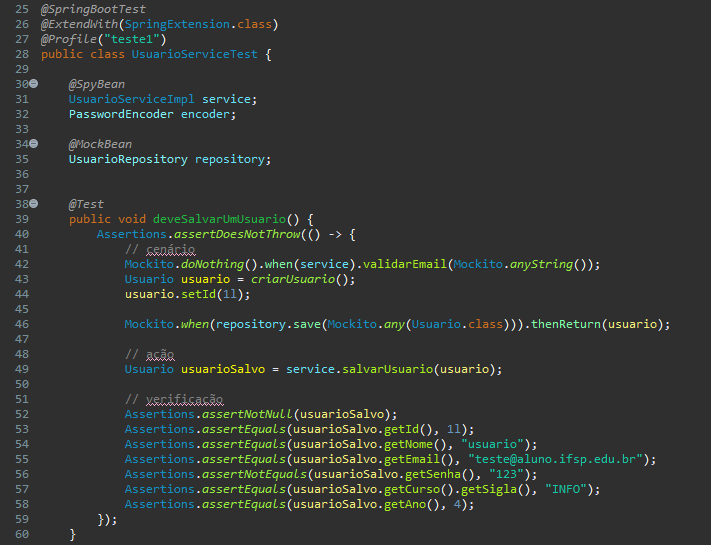
\includegraphics[width=1\textwidth]{anexos/Imagens_Testes/API_teste.png}
\fonte{Os autores}
\end{figure}
\FloatBarrier

Conforme mostrado na \autoref{exemplo teste}, é possível visualizar as anotações ``@SpyBean'' e ``@MockBean'', eles são responsáveis por dizer ao \gls{SpringBoot} quais classes ele deve gerenciar e trazer para dentro do seu próprio contexto. Com a anotação ``@Profile'' é possível definir qual arquivo de propriedades será utilizado, no caso da \autoref{exemplo teste} é o arquivo que contém as configurações para o banco de dados teste.

Já para a cobertura de testes unitários está sendo utilizado o \acs{jacoco}. De acordo com sua documentação, a tecnologia oferece recursos integráveis com o \gls{JUnit}, e o \gls{Eclipse}, \acs{ide} utilizada para construção da \acs{api}. A \autoref{grafico de testes} mostra o gráfico de cobertura de testes, realizado para a classe serviço de pergunta do \gls{ifriends}:

\begin{figure}[htb]
\centering
\caption{\label{grafico de testes} Cobertura de testes}
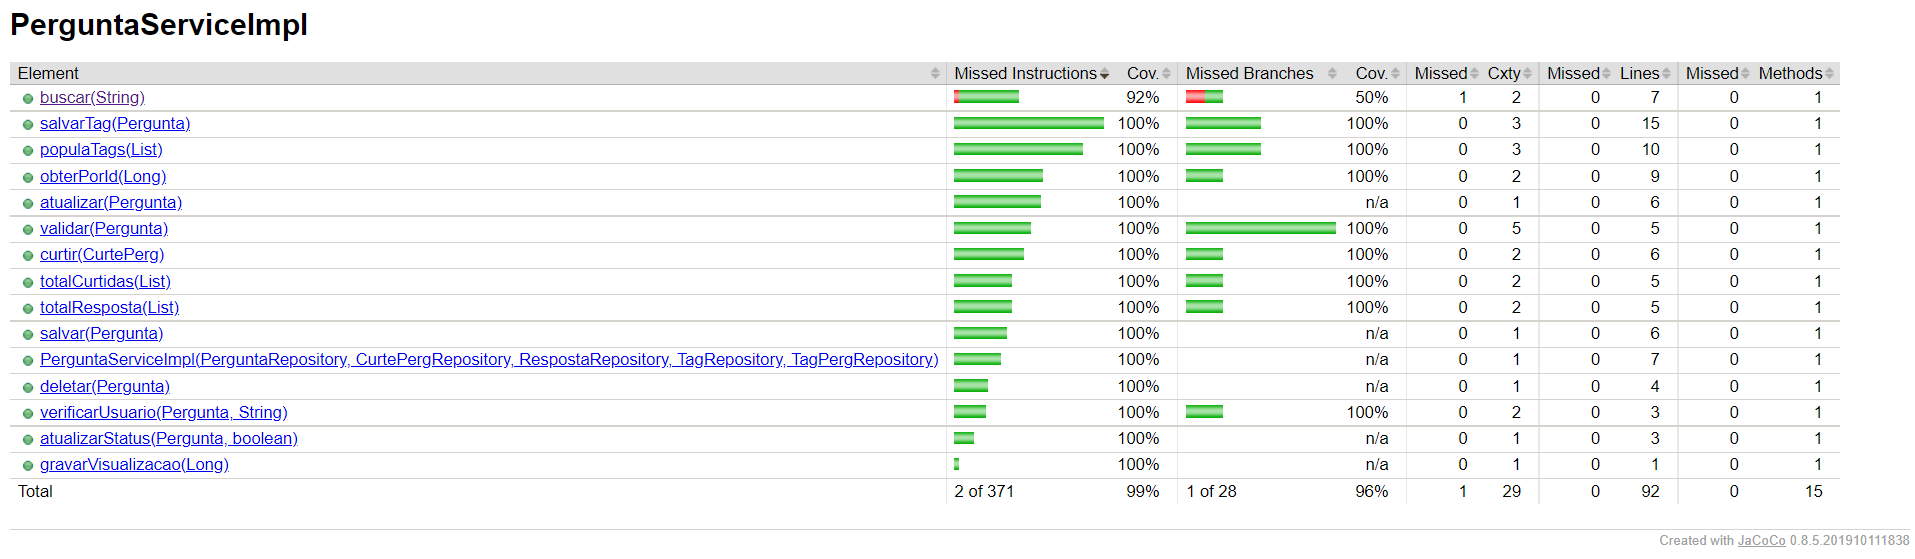
\includegraphics[width=1\textwidth]{anexos/Imagens_Testes/API_grafico-testes.png}
\fonte{Os autores}
\end{figure}
\FloatBarrier

Após a observação feita do gráfico na \autoref{grafico de testes}, a primeira coluna possui os nomes de todos os métodos da classe; a segunda coluna é possível saber a porcentagem total do percurso testado de cada método; a terceira coluna mostra a porcentagem de todas as operações básicas testadas, e o restante das colunas mostram, respectivamente, a quantidade de operações, linhas e métodos da classe.

%--------------------------------------------------------------
\subsection{Testes de usabilidade}
%--------------------------------------------------------------
Segundo \citeonline{alura2022}, testes de usabilidade é uma técnica de caixa-preta qual visa o mapeamento da interação de usuários com o produto de modo a descobrir problemas e pontos de melhorias. 

Na parte de usabilidade, a equipe definiu que, primeiramente, será validada a interface de usuário, verificando se o sistema segue uma coerência baseada nas 10 heurísticas de Nielsen e nos requisitos de acessibilidade especificados no W3C, ou seja, será um teste feito inicialmente pelos próprios desenvolvedores e conforme a frequência de entregas. Ainda para a interface, conforme os requisitos da disciplina,  o sistema deve ser inserido em um validador de interfaces que será especificado nesta documentação, juntamente com seus resultados, após a última entrega - quando finalizados todos os testes com usuários.

%----------------------------------------------------------------
\subsubsection{Cenário de testes}
%----------------------------------------------------------------
Segundo \citeonline{Polo:2020}, um cenário é uma história que descreve a maneira pela qual o sistema pode ser usado, esses cenários devem ser realistas e devem ser testados por usuários reais. Ainda, como características fundamentais, o autor \citeonline{Polo:2020} destaca uma narrativa mais próxima possível da realidade de utilização do sistema, além de ser um cenário de fácil avaliação. 

Dessa forma, para o cenário de teste do projeto \gls{ifriends} serão recrutados cinco estudantes do próprio \acs{ifsp} de forma aleatória, e por meio de uma pesquisa presencial a equipe de \textit{design} deverá cobrir as seguintes etapas: 

\begin{itemize}
%---
    \item \textbf{Introdução amigável:} uma boa introdução, ainda mais sendo ela amigável, deixará o \gls{friend} mais confortável e mais preparado para seguir com a pesquisa. Dessa forma, realizar uma breve introdução informando o motivo da sua presença, qual é a finalidade da pesquisa e informar previamente as ações ele irá realizar é fundamental;
%---    
    \item \textbf{Perguntas consensuais:} como os entrevistados serão os próprios alunos do \acs{ifsp}, esta etapa não será muito complexa. Após realizar a introdução amigável, a equipe de \textit{design} deverá desencadear uma conversa inicial a respeito do assunto que daquela dinâmica deverá seguir, como, por exemplo, realizar perguntas que se relacionem com o projeto ou com sua problemática; 
%---
    \item \textbf{Apresentação da solução:} após envolver o \gls{friend} no assunto, a próxima etapa é mostrar a aplicação, fornecer a possibilidade de ele interagir de fato com o sistema. Se tratando de sua primeira interação, logo de início o \gls{friend} demostrara um certo comportamento, portanto é fundamental que a equipe de \textit{design} identifique essa ``resposta emocional'';
%---
    \item \textbf{Propor desafios:} a próxima etapa da pesquisa é propor desafios para que o \gls{friend} realize na entrevista, dentro desses desafios é importante testar os principais fluxos do sistema. Após concluir todos os desafios planejados, a equipe de \textit{design} pode fazer algumas perguntas sobre a experiência, lembrança, desempenho e precisão; 
%---
    \item \textbf{\textit{Feedback} geral:} por fim, a última da etapa da entrevista refere-se a receber um \textit{feedback} geral por parte do \gls{friend} assim como dar os devidos agradecimentos por sua participação e disposição;
%---
\end{itemize}

Após cobrir os requisitos acima citados, será realizada ainda uma pesquisa de satisfação geral ao final do teste, para verificar a satisfação geral do cliente com relação ao sistema desenvolvido. Vale ressaltar que no \autoref{script_entrevista} podem ser encontrados mais detalhes a respeito da pesquisa.


%------------------------------------------------------------

%------------------------------------------------------------
%--------------------------------------------------------------
\chapter{Histórico de Desenvolvimento}
%--------------------------------------------------------------
Assim como mencionado na \autoref{metodologia agil}, a equipe optou pelo uso da metodologia ágil Scrum, dessa forma o processo de desenvolvimento foi organizado por meio de \glspl{Sprint}, estas foram planejadas a partir das reuniões organizadas entre os membros da equipe. Logo, a seguinte seção visa descrevê-las, assim como apresentar a sua duração.

\begin{itemize}
%---
\item {\textbf{Sprint I: 17/04 a 01/05}}
    
A primeira \gls{Sprint} do projeto em suma visou a inicialização do épico de Gestão de Perguntas, visto que após a realização de estimativas com o \textsl{Scrum Poker} das histórias de usuário, a equipe concordou que este épico era o indicado para dar início ao desenvolvimento do projeto. Dessa forma, foi planejada ainda para a mesma \gls{Sprint} a inicialização da prototipagem das telas, assim como o uma modelagem de dados inicial.
%---
\item {\textbf{Sprint II: 02/05 a 09/05}}
    
A segunda \gls{Sprint} do projeto visou a finalização de dois épicos, isto é, a Gestão de Respostas e a Gestão de Perguntas. Além disso, para esta \gls{Sprint} estava planejada a apresentação da \gls{POC}, logo, também era esperada uma apresentação bem estruturada, assim como o documento de visão/relatório da \gls{POC}. 

Porém, essa \gls{Sprint} não foi concluída completamente, visto que os épicos não foram finalizados com todos os critérios de aceitação prontos, porém foi possível entregar todos os que eram relacionados a construção da \acs{api}. Logo, passamos as tarefas faltantes para a próxima Sprint.
%---
\item {\textbf{Sprint III: 16/05 a 29/05}}
    
Após a apresentação da \gls{POC} do projeto, para a nossa terceira \gls{Sprint} planejou-se realizar os ajustes que ficaram pendentes, sendo na documentação, no \textit{deploy} e na segurança da aplicação. 
%---
\item {\textbf{Sprint IV: 30/05 a 12/06}}
    
Após concluir os ajustes pendentes, para a quarta \gls{Sprint} se planejou estabelecer de vez uma boa conexão com a API no \textsl{\gls{front-end}} para que todas as requisições do épico de Gestão de Perguntas e o épico de Gestão de Respostas tenham um bom resultado, utilizando a autenticação do usuário. Na parte da documentação se planejou fazer a organização do documento, assim como atualizar as modificações realizadas no desenvolvimento até o momento. 
%---
\item {\textbf{Sprint V: 12/06 a 20/06}}

Devido aos contratempos encontrados na disciplina de \acs{pds} foi possível criar uma \gls{Sprint} extra antes da primeira apresentação parcial, logo, a quinta \gls{Sprint} visou à finalização e melhoria das tarefas pendentes da \gls{Sprint} anterior assim como a preparação da apresentação do projeto. 
%---
\item \textbf{{Sprint VI: 31/07 a 21/08}}

A sexta \gls{Sprint} do projeto teve foco em efetuar a revisão do \textit{backlog} e realizar os ajustes necessários na documentação visando a entrega final. Além disso, a aplicação \textsl{\gls{front-end}} foi hospedada no \gls{vercel} e finalizamos as partes faltantes como a prototipação e a revisão de literatura. Vale ressaltar também que devido à revisão do \textit{backlog} foi possível desenvolver um plano de entregas (\autoref{plano_entrega}).
%---
\item \textbf{{Sprint VII: 21/08 a 04/09}}
A sétima \gls{Sprint} prevê a entrega da documentação, anteriormente desenvolvida, o desenvolvimento do projeto, conforme as histórias de usuários definidas, assim como realizar a preparação da apresentação final.

\item \textbf{{Sprint VIII: 04/09 a 26/09}}
A oitava \gls{Sprint} teve foco no desenvolvimento e na testagem das funcionalidades previstas para a apresentação final da aplicação, utilizando das definições previstas nos refinamentos para finalizar o que havia sido planejado. 

\item \textbf{{Sprint IX: 26/09 a 07/11}}
A nona \gls{Sprint} foi reservada para ajustar os problemas apontados na documentação do projeto, refinar as histórias para o desenvolvimento, executar os testes de usabilidade e realizar a última entrega do documento. 

\item \textbf{{Sprint X: 07/11 a 28/11}}
A última \gls{Sprint} foi planejada para o desenvolvimento dos ajustes na aplicação e dos últimos detalhes faltantes para a entrega final, bem como a mudança de alguns itens com base no retorno dado pelos usuários. Além disso, também se restringiu a inclusão dos últimos vídeos no canal do YouTube e à apresentação das mudanças realizadas desde a entrega final. 

\end{itemize}

% -------------------------------------------------------------
%--------------------------------------------------------------
\section{Descartes}
%--------------------------------------------------------------
A seguinte seção foi criada visando fornecer informações a respeitos dos descartes realizados a partir do espoco inicial proposto para o projeto. 

O primeiro descarte a ser feito foi em relação ao uso do \gls{scoold} no desenvolvimento, inicialmente a equipe pretendia fazer uso dessa plataforma visto que as funcionalidades que ela trazia se assemelhavam a boa parte do que se pretendia desenvolver no \gls{ifriends}. 

Mas, após fazer os estudos iniciais a respeito de como fazer essa implementação e de como fazer a integração com os outros recursos que ainda precisariam ser desenvolvidos, a equipe denotou que a tarefa se tornaria mais complexa do que o esperado, já que era necessário um estudo mais aprofundado, e como não dispomos um tempo de desenvolvimento significativo decidiu-se usar o \gls{scoold} apenas como uma inspiração. Vale lembrar que o descarte da plataforma já tinha sido previsto no escopo inicial do projeto, então o tempo aplicado no estudo não foi perdido e se tomou como aprendizado.

Outro descarte/problema que enfrentamos foi a inexistência da seção de testes unitários no \gls{front-end}, tendo em vista que pecamos com planejamento para a sua inclusão desde o início do desenvolvimento, e, por este motivo, não conseguimos incluir a porcentagem de cobertura de testes, com a inclusão da biblioteca JEST no ReactJS, a tempo da entrega final deste documento, porém é possível executar os testes através do comando especificado na documentação do projeto (arquivo .md) descrita dentro do repositório da equipe no sistema de versionamento de código escolhido, disponível na pasta \textsl{ifriends-web}.

Vale ressaltar que, esse último descarte, poderia motivar, por exemplo, a escolha de um modelo de trabalho no \gls{front-end} que pudesse facilitar a construção dos testes sem muitas dificuldades, seja com a adesão de algum \gls{framework2} específico que trouxesse isso por padrão, ou com a utilização de metodologias como o desenvolvimento orientado a testes.

 
%--------------------------------------------------------------
 \section{Mudanças}
%--------------------------------------------------------------
Visando também pelas mudanças, a seguinte seção tem o intuito de apresentá-las seguida dos critérios considerados para a sua aplicação no projeto. 
 
A primeira mudança mais evidente foi realizada sobre o \gls{heroku} em relação ao \gls{front-end} do sistema: após várias investigações realizadas pela equipe, foi encontrado o \gls{vercel} como melhor opção de servidor de hospedagem para substituir o \gls{heroku}, visto que ele atendia todos os \href{https://vercel.com/blog/automatic-ssl-with-vercel-lets-encrypt}{requisitos de segurança faltantes}, além de que foi constatado pela equipe posteriormente que o \textsl{Buildpack} utilizado para subir a aplicação no \gls{heroku} seria \href{https://github.com/mars/create-react-app-buildpack}{descontinuado}, o que também contribuiu para a mudança. Para o \gls{back-end}, por outro lado, tentou-se encontrar um serviço de hospedagem que cumprisse todos os requisitos existentes no \gls{heroku}, mas não se obteve sucesso na busca. Como os requisitos de segurança foram cumpridas de forma satisfatória, a equipe considerou que não seria considerado urgente mudar a hospedagem da \gls{api} neste momento.

Por último, precisamos mudar também a quantidade total de estudantes a serem entrevistados no nosso plano de testes, tendo em vista que o número estipulado inicialmente não comportou a agenda que os integrantes da equipe tinham disponível, pois as entrevistas feitas duraram mais tempo do que imaginamos e, portanto, a quantidade original se tornou inviável. De todo modo, disponibilizamos a pesquisa de \acs{nps} para que possamos centralizar os \textit{feedbacks} dados e ainda manter o processo de melhoria contínua com base nela, sem descartar a possibilidade de realizar eventuais entrevistas no futuro.
% -------------------------------------------------------------
%------------------------------------------------------------
